\chapter{Methods}
\label{sec:Methods}
Although the particle filter  is a standard Regularized
Particle filter, as described in \cite{Arulampalam2002a}, optimizing the 
particle filter for use with FMRI data is non-trivial. 

\section{Prior Distribution}
\label{sec:PriorDist}
For the BOLD model described in \autoref{sec:BOLD Physiology}, several
different studies have endeavored to calculate parameters. The results
of these studies may be found in \autoref{tab:Params}, and the methods 
used for each may be found in \autoref{sec:Prior Works}. Unfortunately,
\cite{Friston2000} only studied regions deemed active by the General 
Linear Model; and most other research (including \cite{Friston2001}) used these results as 
the source for their priors. 
The one exception is \cite{Johnston2008}, which came to a extremely different
distributions. For a particle filter, the choice of a prior is
the single most important design choice. A very wide prior will require
more particles to be sufficiently dense, a very thin prior may miss
the true parameters. Consequently, for this work it was natural
to use priors that will give results consistent with similar tests. accepted result,
\cite{Friston2000}. This constrains the usefulness of the model to
areas that fall within the prior distribution, yet will allow results
to be comparable to other works. There is a significant need for better
estimates of the physiological parameters; and, while physical experiments
may not be possible, it would not be unreasonable to do a study with
exhaustive simulated annealing or hill climbing tests for multiple
regions and multiple patients. The purpose for this work is to determine
the fitness of particle filters for this task. Ultimately this algorithm may become
more useful as more studies are done on BOLD model that don't require
priors. 

There is an interesting anomaly with the priors found in virtually all
the works that characterized the parameters, except \cite{Johnston2008}.
The BOLD signal is universally recognized to be around $2-3\%$, maybe
reaching $5\%$ in extreme activation. Yet using the mean priors
from \cite{Friston2000}, the signal response for a $.1$ second
impulse only reaches maybe half a percent, as \autoref{fig:MeanResponseF}
shows.

\begin{figure}
\centering
\label{fig:MeanResponseF}
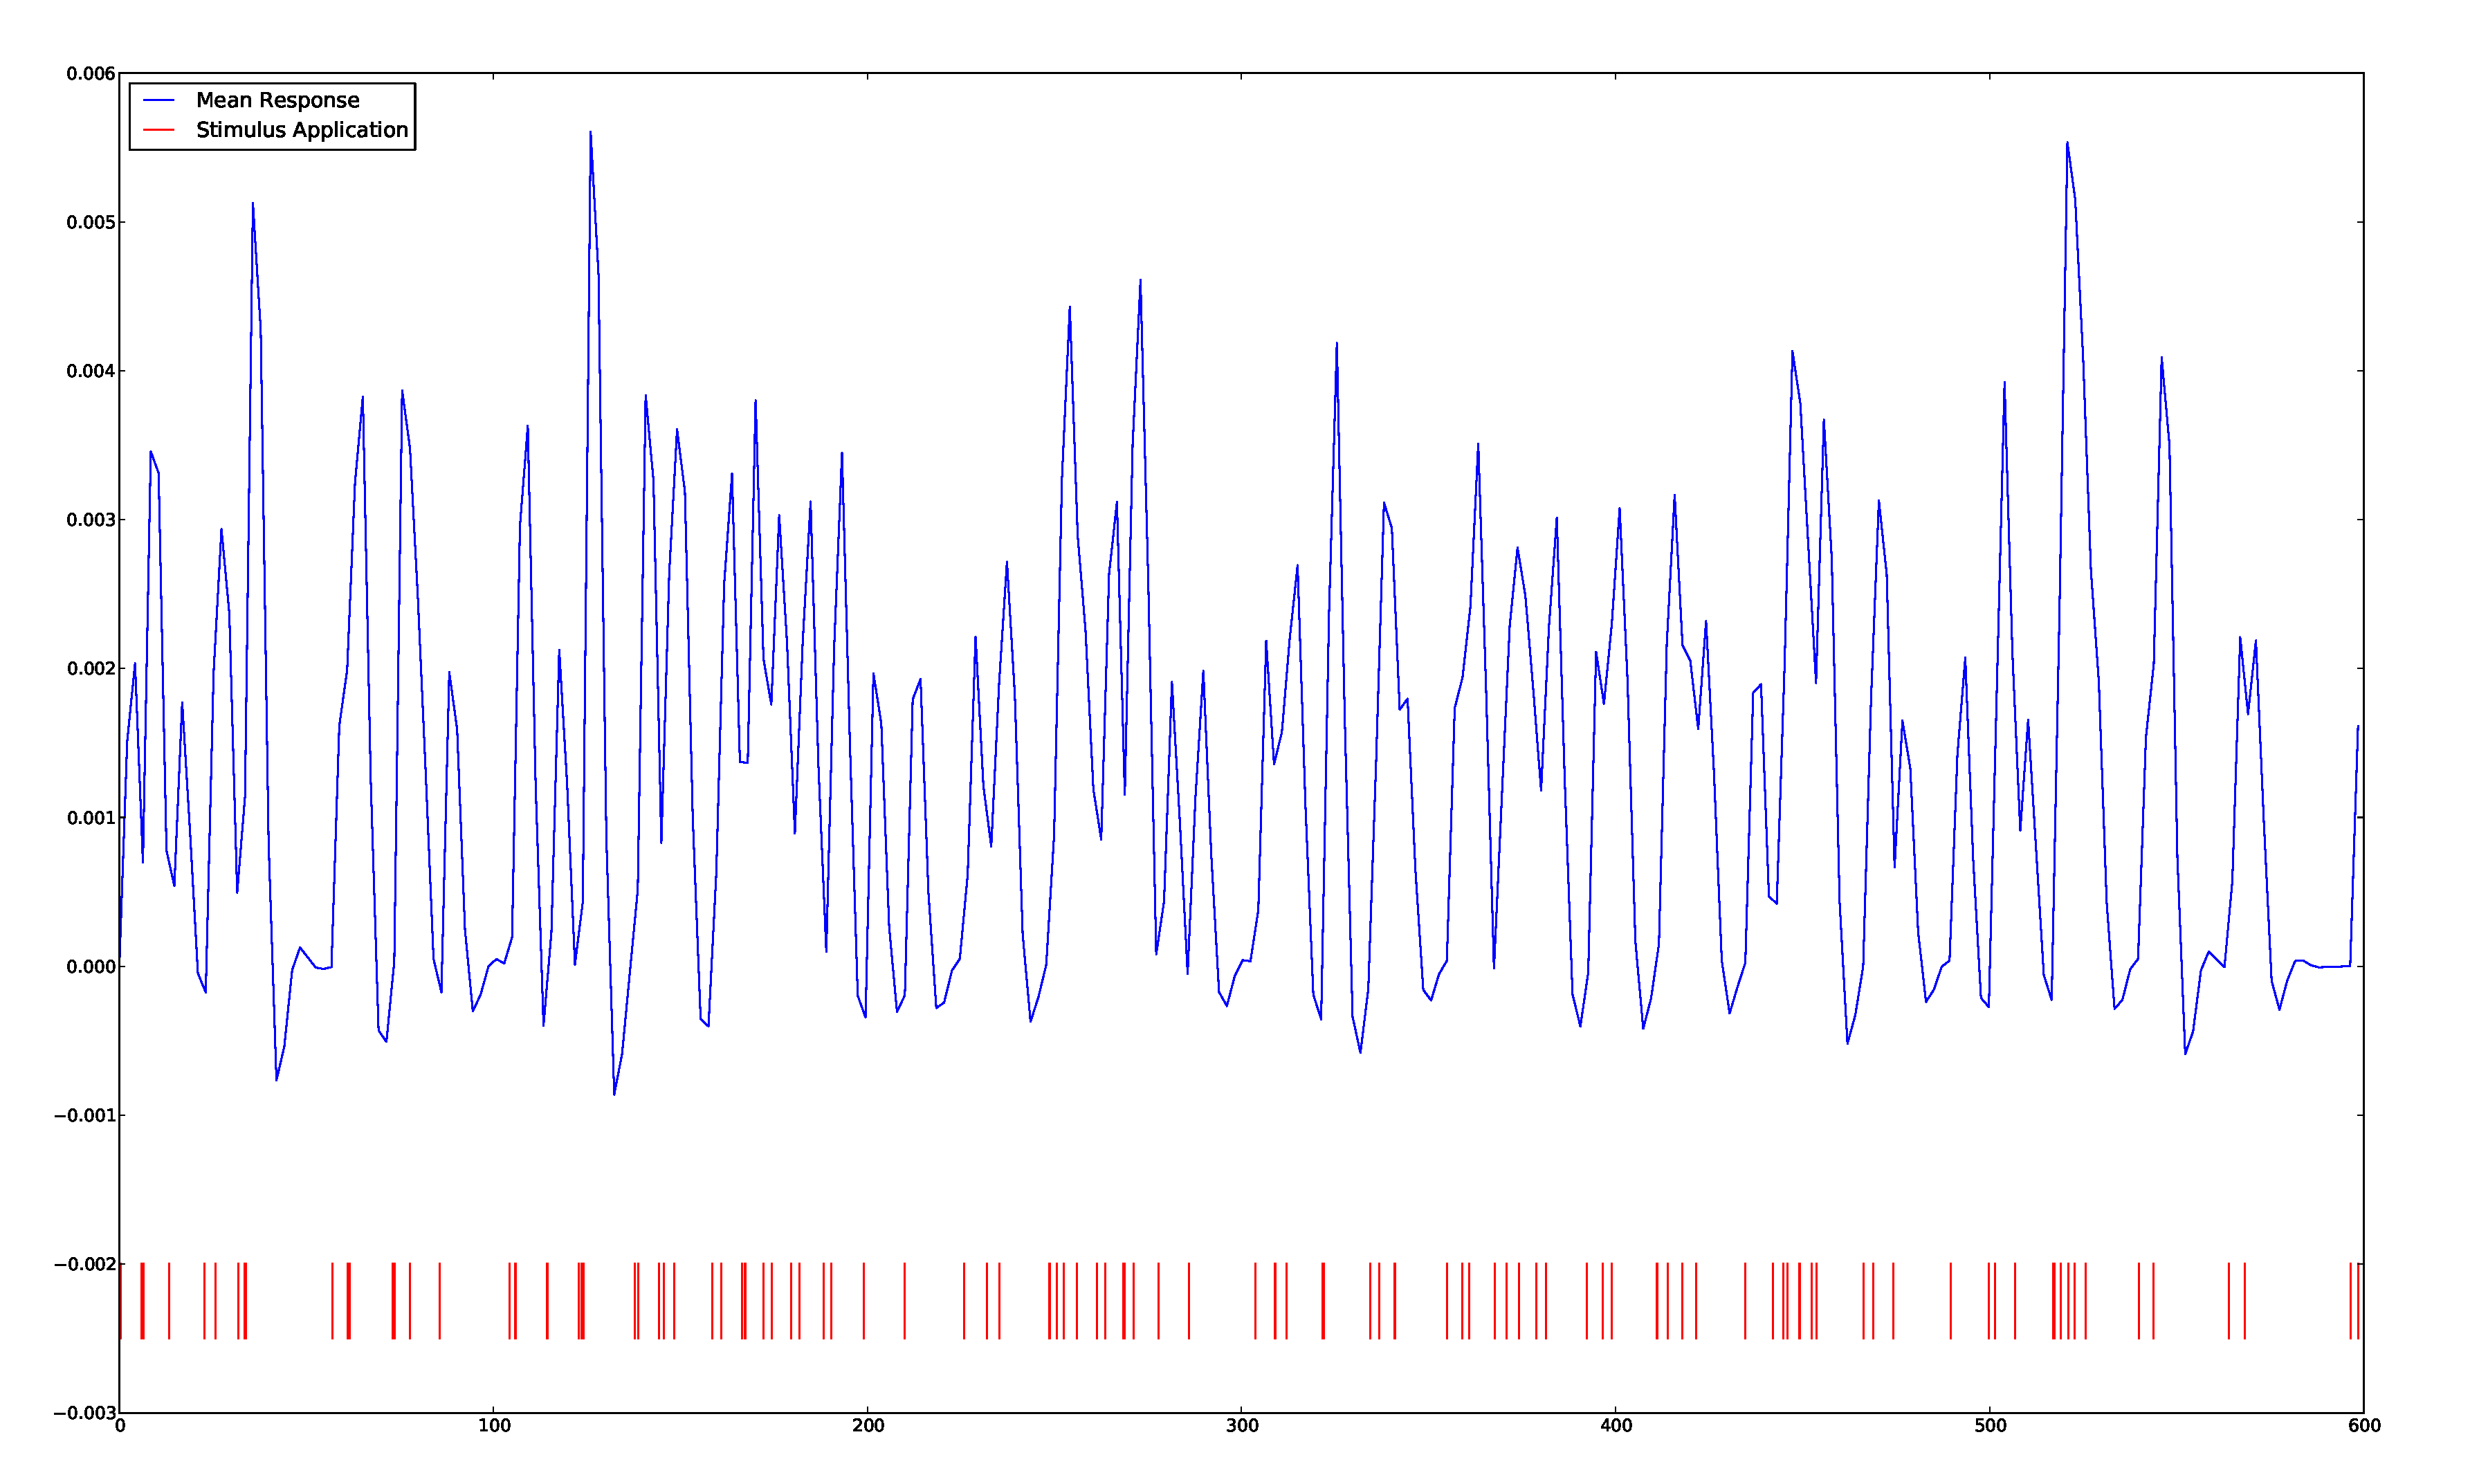
\includegraphics[trim=6cm 3cm 6cm 3cm,width=16cm]{images/mean_response}
\caption{Response to $.1s$ impulses with the mean parameters from \cite{Friston2000}}
\end{figure}

While this could be the result of a stimulus
being too short to lead to strong activation, a similar stimulus
scheme in real data showed a much larger response than 
half a percent as well. In fact, after applying de-trending,
converting the image to percent-difference, and removing 
outliers ($ BOLD > 10\% \text{ or } BOLD < -10\%$) the total variance
across all \emph{active} voxels was still around .02, indicating
that in active voxels a signal peaking below .005 seems unlikely. 
Of course, if more restriction were placed on the outliers, its possible
this standard deviations could be brought down. 
The parameter estimates by \cite{Johnston2008} are even more 
confusing, with peaks of well below $.1\%$ (\autoref{fig:MeanResponseJ}).

\begin{figure}
\centering
\label{fig:MeanResponseJ}
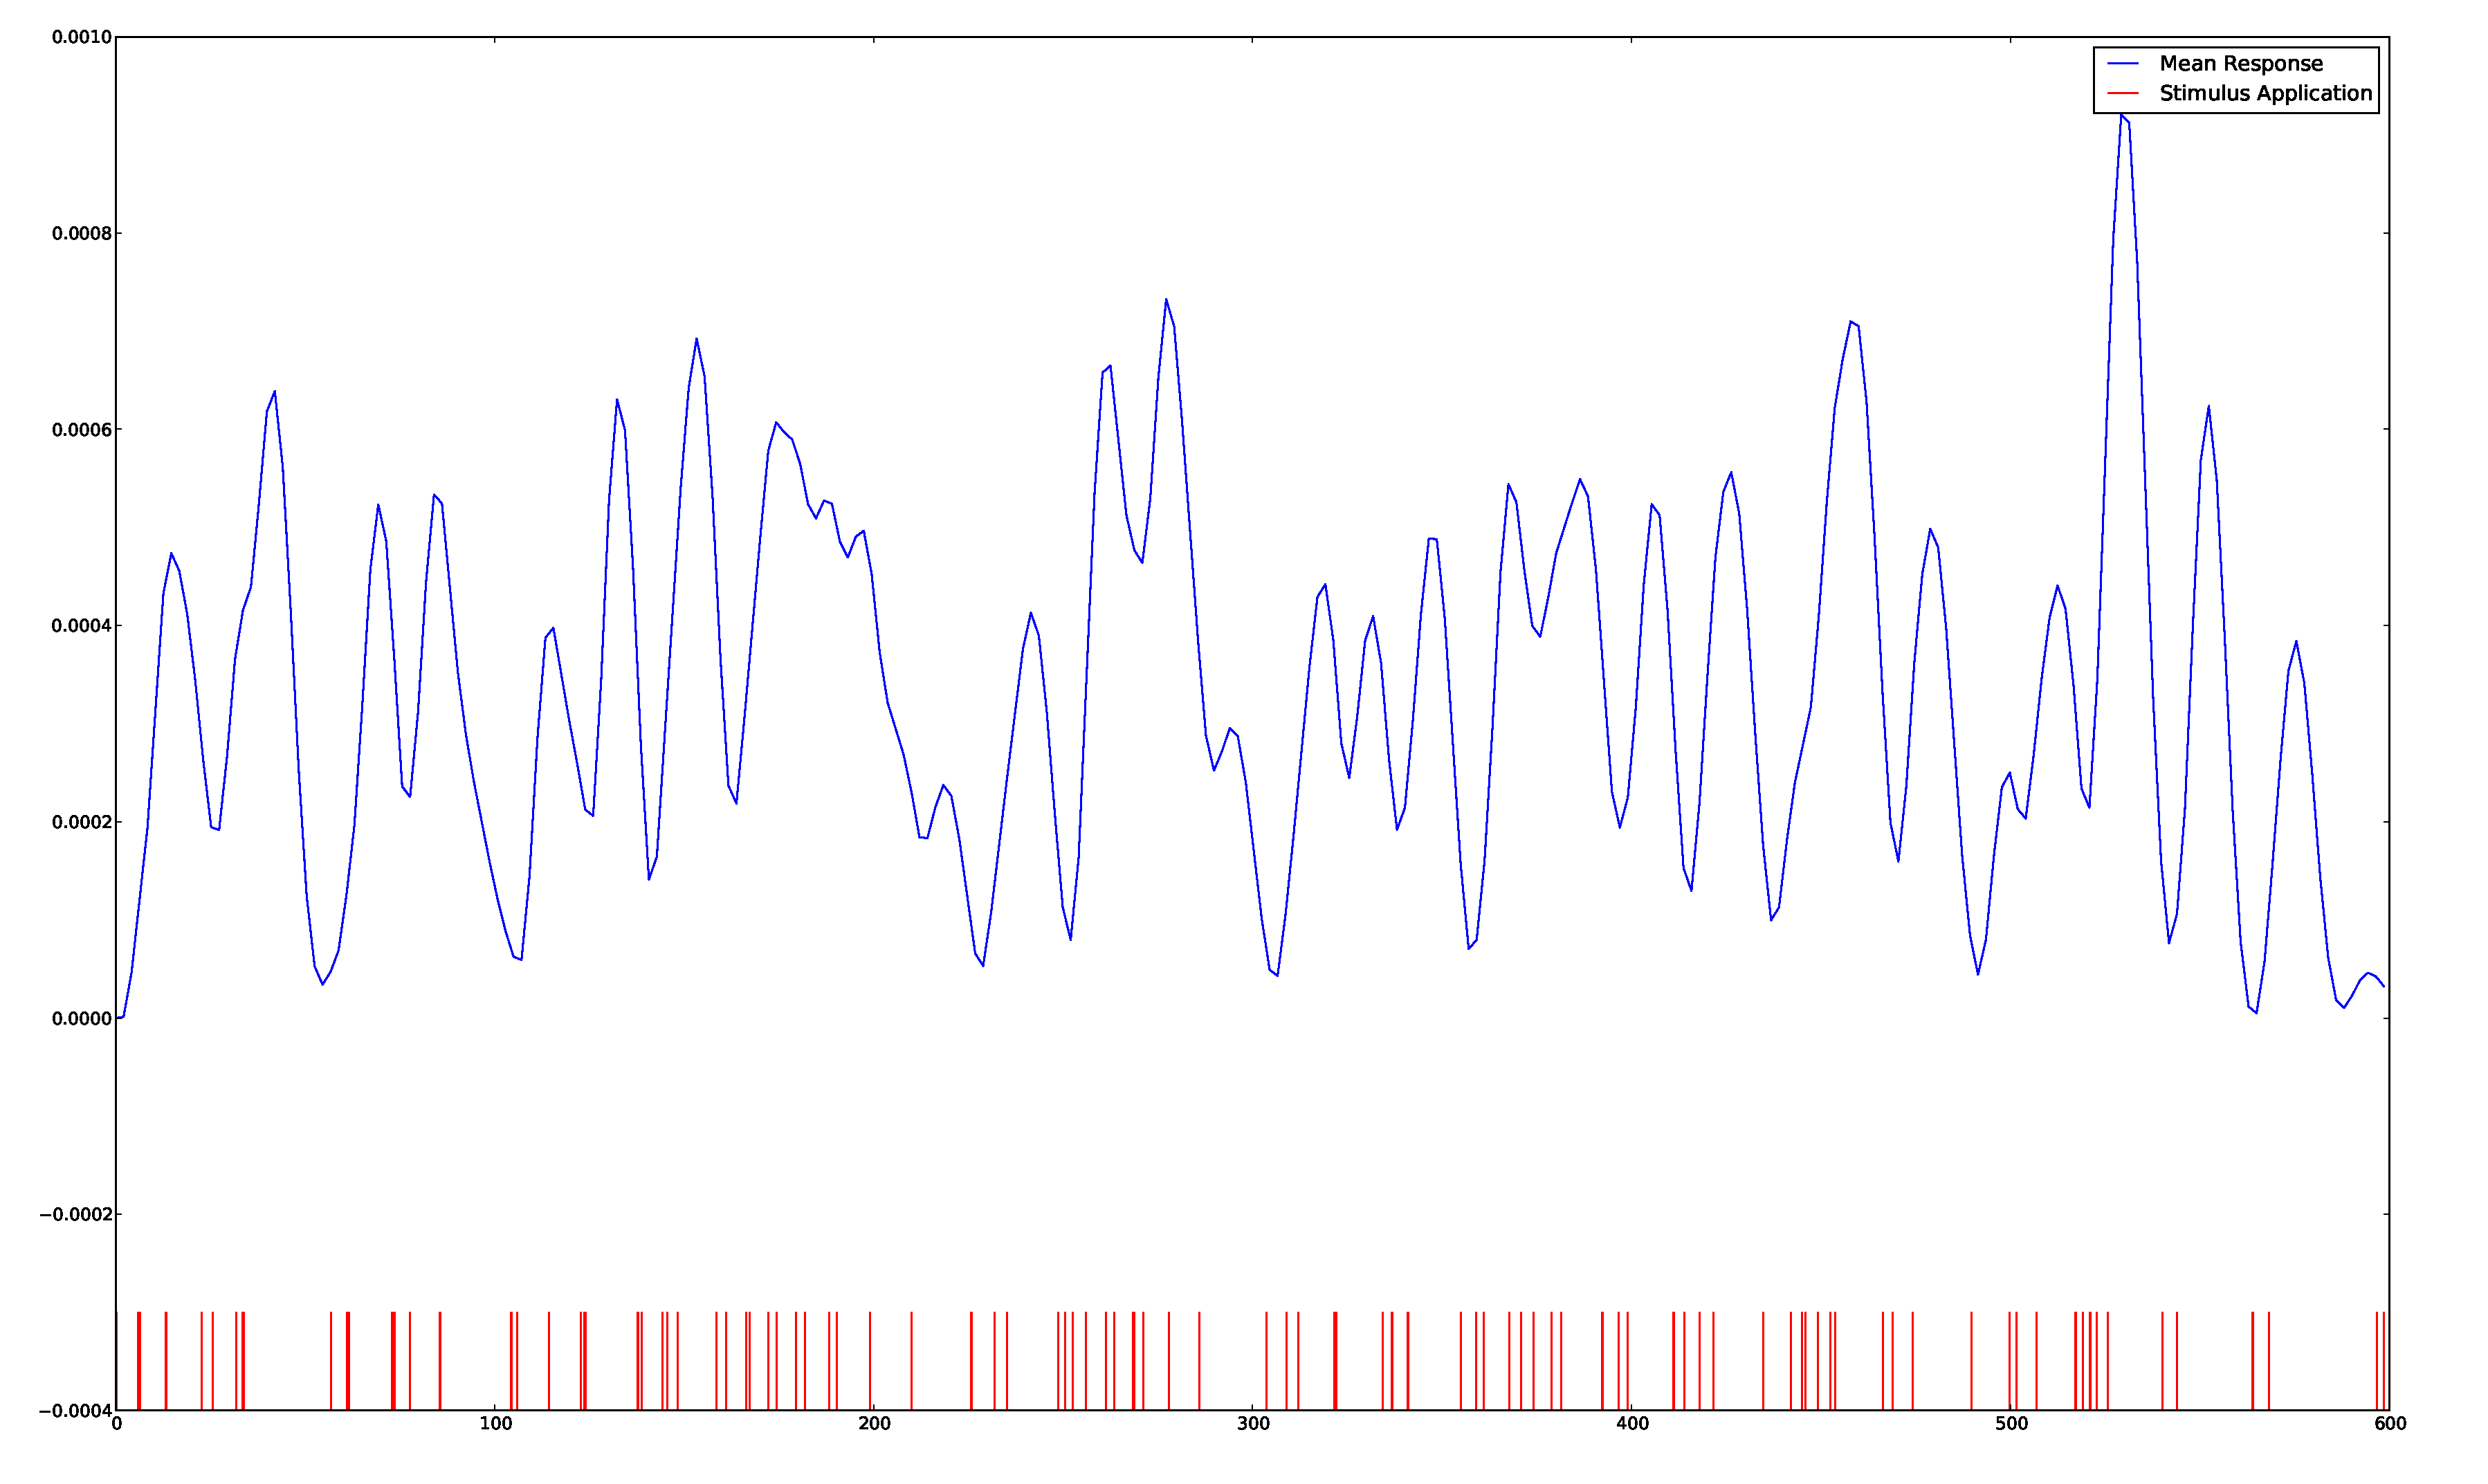
\includegraphics[trim=6cm 3cm 6cm 3cm,width=16cm]{images/mean_response_johnston}
\caption{Response to $.1s$ impulses with the mean parameters from \cite{Johnston2008}}
\end{figure}

Its likely that these differences are due to some difference in preprocessing,
although in \cite{Deneux2006} the signals were found to be peaking around
$1\%$, unlike \cite{Friston2000} which shows signals peaking at up to
$3\%$ or $4\%$. In my own tests, it seemed necessary for $\epsilon$ to
reach well over $1.5$ and $V_0$ to reach more than $.4$ to reach these
peaks; of course other methods may be equally able. 
Therefore, to account for these discrepancies, somewhat broader
distributions are used than the numbers used in \cite{Friston2000}
(which are widely used, \cite{Hu2009}). The 
priors used in the particle filter may be found in \autoref{tab:Prior}.

\begin{table}[t]
\centering
\begin{tabular}{|c || c | c | c |}
\hline 
Parameter & Distribution & $\mu$ & $\sigma$ \\
\hline
$\tau_0$ & Gamma & .98 & .25 \\
$\alpha$ & Gamma & .33 & .045\\
$E_0$    & Gamma & .34 & .03  \\
$V_0$    & Gamma & .04 & .03 \\
$\tau_s$ & Gamma & 1.54  & .25\\
$\tau_f$ & Gamma & 2.46  & .25\\
$\epsilon$ & Gamma & .7  & .6 \\
\hline
\end{tabular}
\caption{Prior distributions used in the particle filter.}
\label{tab:Prior} 
\end{table}

Note that although the mean remains the same for all the 
parameters other than $\epsilon$, the standard deviation is set
much higher to account for the disagreement between studies
(\autoref{tab:Params}). 
Because all the parameters are taken to be strictly positive, and the
standard deviations are approaching the mean, I used a gamma distribution.
This prevents the Gaussian from placing parameters in the nonsensical 
territory of negative activation, or negative time constants.

Another aspect of the prior is using enough particles to get a 
sufficiently dense approximation of the prior. For 7 dimensions,
getting a dense prior is difficult. Insufficiently
dense particles will result in inconsistent results, of course the
processing time will scale up directly with the number of particles.
A dense initial estimate is important so that some particles land
near the solution; but as the variance decreases the number of 
particles needed decreases as well. Thus, as a heuristic, initially
the number of particles is set to 28,000, but after resampling,
the number of particles is dropped to 1,000. Typically during the 
first few measurements the variance drops precipitously since most particles
don't describe the system well. The particles that are left are in a
much more compact location, allowing them to be estimated with 
significantly fewer particles. These numbers aren't set in stone,
and depending on the complexity of the system or desired accuracy
they could be changed; however, they seem to be the minimum that
will give consistent results.

\section{Model}
As originally written in \autoref{sec:BOLD Physiology} the state variables
for the BOLD model are as follows:
\begin{eqnarray}
\dot{s} &=& \epsilon u(t) - \frac{s}{\tau_s} - \frac{f - 1}{\tau_f} \\
\dot{f} &=& s\\
\dot{v} &=& \frac{1}{\tau_0}(f - v^\alpha)\\
\dot{q} &=& \frac{1}{\tau_0}(\frac{f(1-(1-E_0)^f)}{E_0} - \frac{q}{v^{1-1/\alpha}})
\end{eqnarray}
The original assumption regarding particle filter models (\autoref{sec:Particle Filter Model})
included noise in the update of $x$, however that is not included here.
The reason for the difference is that cloud of particles is, to some extent,
able to model that noise. It is common, however, to actually model that noise
in particle filters by adding a random value to each updated state variable. 
Because the purpose of this particle filter is to learn the underlying distribution
of the static parameters, rather than precisely model the time course of the 
in the dynamic parameters ($\{s,f,v,q\}$) this noise is left out. Because the
BOLD model is dissipative, when no stimuli are applied, all the particles 
will decay to ($\{0,1,1,1\}$) which they should. If evolution noise were added, the 
particles would then weight particles based on the results of that noise, rather
than on the quality of the static parameters. Typical particle filters 
also use this state noise as an exploratory measure; however this method is
less well suited when the system is dissipative. 

Thus, at each time step, the states were linearized, and each state variable,
$s$, $f$, $v$, $q$, were changed according their previous rate of change.
Because of the difficulty of solving a system of nonlinear equations, I 
did not use the typical Runge-Kutta 4/5 technique to optimize step sizes. 
The cost of missing a feature in these differential equations typically leads
to non-real numbers shortly down the road. Because the non-real numbers do 
not come until the solution has had the chance to update two or three more
times, taking long steps can result in catastrophic and un-recoverable errors. 
Typically a step size of .001 was used, after finding that even .01 can
at times lead to the state equations careening out of control.

\section{Resampling}
\label{sec:Resampling}
The algorithm for resampling is described in \autoref{sec:Particle Filter Resampling}.
The primary design decision for resampling is the regularizing
kernel. As mentioned previously, the Gaussian kernel is convenient,
because it is simple to sample from. As discussed in \autoref{sec:Particle Filter Resampling},
as long as resampling is kept as a last resort, some amount of over-smoothing
won't impair convergence. Therefore, for this work I chose a Gaussian kernel of
bandwidth equal to the original distribution's covariance. Obviously this will
apply a rather large amount of smoothing to the distribution; however, on average
resampling is only applied every 20 to 30 measurements, and because randomization
is being applied to model updates this gives the filter some mobility. 

Because the regularized resampler will almost certainly over-smooth,
it is necessary to wait until the $N_{eff}$ drops relatively low
(say below 25) before resampling is performed. As an additional 
measure against sharp drops in the $N_{eff}$ that may quickly raise
back up, resampling is only performed when two consecutive low
$N_{eff}$'s are found. 
The danger in waiting longer to resample is that if there were no
particles in the vicinity of the solution, then particle deprivation
can occur.  When this happens, the resampling
stage will have an inappropriately small variance which will lead to an 
inappropriately small support for the distribution. After this, the 
distribution will be unrecoverable. Thus, when the $N_{eff}$ gets down
to extremely low values (below 5), usually this is an indication of particle
deprivation; something that is also usually accompanied by 
fast drops in variance. When this happens, it is often preferable 
to return to a previous, wider estimate of scale for the regularization
and continue from there. Thus to keep particle deprivation from 
affecting the results; a previous covariance matrix is 
used as the regularization bandwidth. In my algorithm I use
the last covariance matrix for which the $E_{eff}$ was greater than
the threshold. This guarantees that there was at least some amount of 
particle diversity, and also helps prevent converging prematurely.

When some sort of particle deprivation has not occurred, regularized
resampling with a large bandwidth will slow down convergence. Thus
as mentioned previously, to prevent over smoothing, the particle
filter algorithm used here waits until 
the effective sample size drops below 25 for two measurement points
in a row. This seemed to give good results, and avoids
temporary drops in the $N_{eff}$ caused by outliers. 

\section{Choosing $P(y_k | x_k)$}
\label{sec:Methods Weighting Function}
Choosing a representation of an unknown distribution tricky, and while
the usual choice is a Gaussian distribution, there are reasons why it
may not be the best.  Studies of the noise in FMRI typically characterise
noise as an additive noise process with Gaussian steps; a Wiener process. 

As noted in \autoref{sec:Introduction Noise}, the noise is not strictly Gaussian,
nor is it strictly Wiener. As with any unknown noise however, it is necessary 
to make some assumption. If the weighting function ($P(y_k | x_k)$) exactly
matches the measurement error, then the ideal particle filter will result.
Particles with $x_k$'s that estimate $y_k$ far out on the weighting
function will quickly have weights near 0. Thus, an weighting function that
exactly matches $P(Y(t) | X(t))$ will easily, and correctly throw out incorrect
particles. However assuming that this function is not going to be found 
for arbitrary voxels, it is necessary to choose a function to approximate this 
probability. The cost of choosing an overly broad distribution for this
function is an overly broad $P(x_k | y_k)$; and ultimately an overly
broad $P(x_k | y_{0:k})$. On the other hand, an overly thin distribution
will lead to, at best, an overly thin representation of these same 
distributions; but at wost will lead to particle deprivation (all particles
being zero-weighted). If the \emph{true} distribution were found, particle
deprivation would indicate that that time series is not being affected
in any way describable by the prior distribution/model. Particle deprivation
due to an under-variant weighting function gives no information. Thus,
the cost of a under estimating variance is higher; a fact that definitely needs
to be taken into account. 

Because of the need to err on the side of caution I tested several weighting
functions. In addition to the Gaussian I also tested the Laplace and Cauchy
distributions, both of which have much wider tales than the Gaussian. The
benefit of the wider tailed distributions is that they don't down-weight
particles quite as fast. Additionally, the Laplace distribution has the
benefit of having a non-zero slope at the origin. This means that even
if the distribution is made overly broad, it will still distinguish between
particles that are near the origin.

After trial and error, I chose the weight standard deviation to be $.005$. Obviously
the case of the Cauchy, this is simply the scale parameter. While I 
did attempt to automatically set the standard deviation, I found that the algorithm
became too unpredictable. Essentially, if the weight function isn't
fixed across voxels, very noisy time series with no actual signal will 
converge to nonsensical results. 
In the future, it may be possible to set the standard deviation by
taking a small sample from resting data and using the sample standard deviation.
Since this is the first attempt at using particle filters for modeling the 
BOLD model, in this work I set the standard deviation manually at $.005$,
because it gives a more consistency and control. 

\section{BOLD Noise}
\label{sec:Introduction Noise}
As demonstrated in \autoref{sec:BOLD Physiology} the BOLD response has been
extensively studied and despite minor discrepancies, the cause of the BOLD 
signal is well known. However, as FMRI detects an  
aggregate signal over the space of cubic centimeters, there are
plenty of sources of noise. Though local neurons act
together (i.e. around the same time), the density of neurons, the
density of capillaries, and slight differences in activation across 
a particular voxel can all lead to signal attenuation and noise. 

A particularly difficult form of noise present in FMRI is a low frequency
drift, often characterized as a Wiener process (\cite{Riera2004}). 
Though not present in all regions, as much as ten to fifteen percent
of voxels can be affected (\cite{Tanabe2002}), thus it is prevalent enough to cause significant
inference problems \cite{Smith2007}. It is still not
clear what exactly causes this noise noise comes from, although it is possible it is 
the result of magnets heating up, or some distortion in magnetic
fields \cite{Smith2007}. It is clear that this drift signal is not solely
due to a physiological effects, given its presence in cadavers and phantoms 
\cite{Smith1999}. Interestingly, it is usually spatially correlated, and
more prevalent at interfaces between regions, though 
by no means limited to such areas. Though one potential source
could be slight movement, given that co-registration of volumes to a single time
point is standard, this is unlikely. Regardless, the problem mandates
the use of a high pass filter to make inference reasonably powered
\cite{Smith2007}.

In order to characterize the noise, I analyzed resting state data.
During resting state, the patient is shown no images, and he is asked
to avoid movement and complex thought, to the best of his abilities.
Some limitations exist, for instance EPI sequences are noisy
which could cause some stimulus in the auditory cortex, and of course
long sequences could give the patient time for his mind to wander.
Overall though there should be no activation, and thus the signal will
consist entirely of noise. Therefore resting state data is perfect
for analyzing the noise distribution. The locations were chosen from
points all around the brain, all in grey matter voxels. The time
series were also chosen because they were representative of different types
of noise I found in the resting state data.

Because most methods (including the one used in this paper)
assume the noise realizations are independent of each other, the auto-
correlation is of particular interest (which is a necessary but not
sufficient condition for independence). Gaussianity is also a common
assumption made in studies of FMRI data, though that assumption is not
made in this work. Regardless, comparing the distribution to a Gaussian
is informative, so I used Q-Q plots to compare example data with the
Normal distribution. Additionally, in FMRI data the noise is often considered 
to be Wiener \cite{Riera2003}. Recall that a Wiener random process is
characterized by steps that are Gaussian; in other words the difference between
any two samples is Normally distributed. The simulations discussed in 
\autoref{sec:Single Voxel Simulation} make use of this, 
by adding a Wiener random process to the overall signal. To determine
whether the noise is in fact Wiener, the distribution of 
the difference between adjacent measurements was plotted against
a Gaussian. Wiener processes further assume that the steps are independent;
so the steps should have near flat autocorrelation functions.

Finally, removal of the drift is often
performed with some variation of a high pass filter, 
so I checked the noise distribution after applying such a filter (in
this case the subtraction of a spline, see \autoref{sec:Methods Preprocessing}).
Here I wanted to know how effective my high pass filter at the removal of
Wiener noise.

\autoref{fig:QQDC} shows the 
results with a regression line fit to the points on the Q-Q plot.
Recall that in a Quartile-Quartile (Q-Q) plot, if the points plotted on the 
x-axis and the points
on the y-axis come from the same \emph{type} of distribution then all the points will
fall on a line. Differences in the variance will cause the line to have a slope
other than 1, while differences in the expected value will cause the fitted line
to be shifted. In these Q-Q plots, the points are being compared to the standard
Gaussian distribution, so the quality of the line fit determines how closely the points
fit the Gaussian distribution. Note that in \autoref{fig:QQDC} the points have all been 
normalized (changed to percent difference).
\begin{figure}
\centering
\subfigure[]{\label{fig:QQDC:A}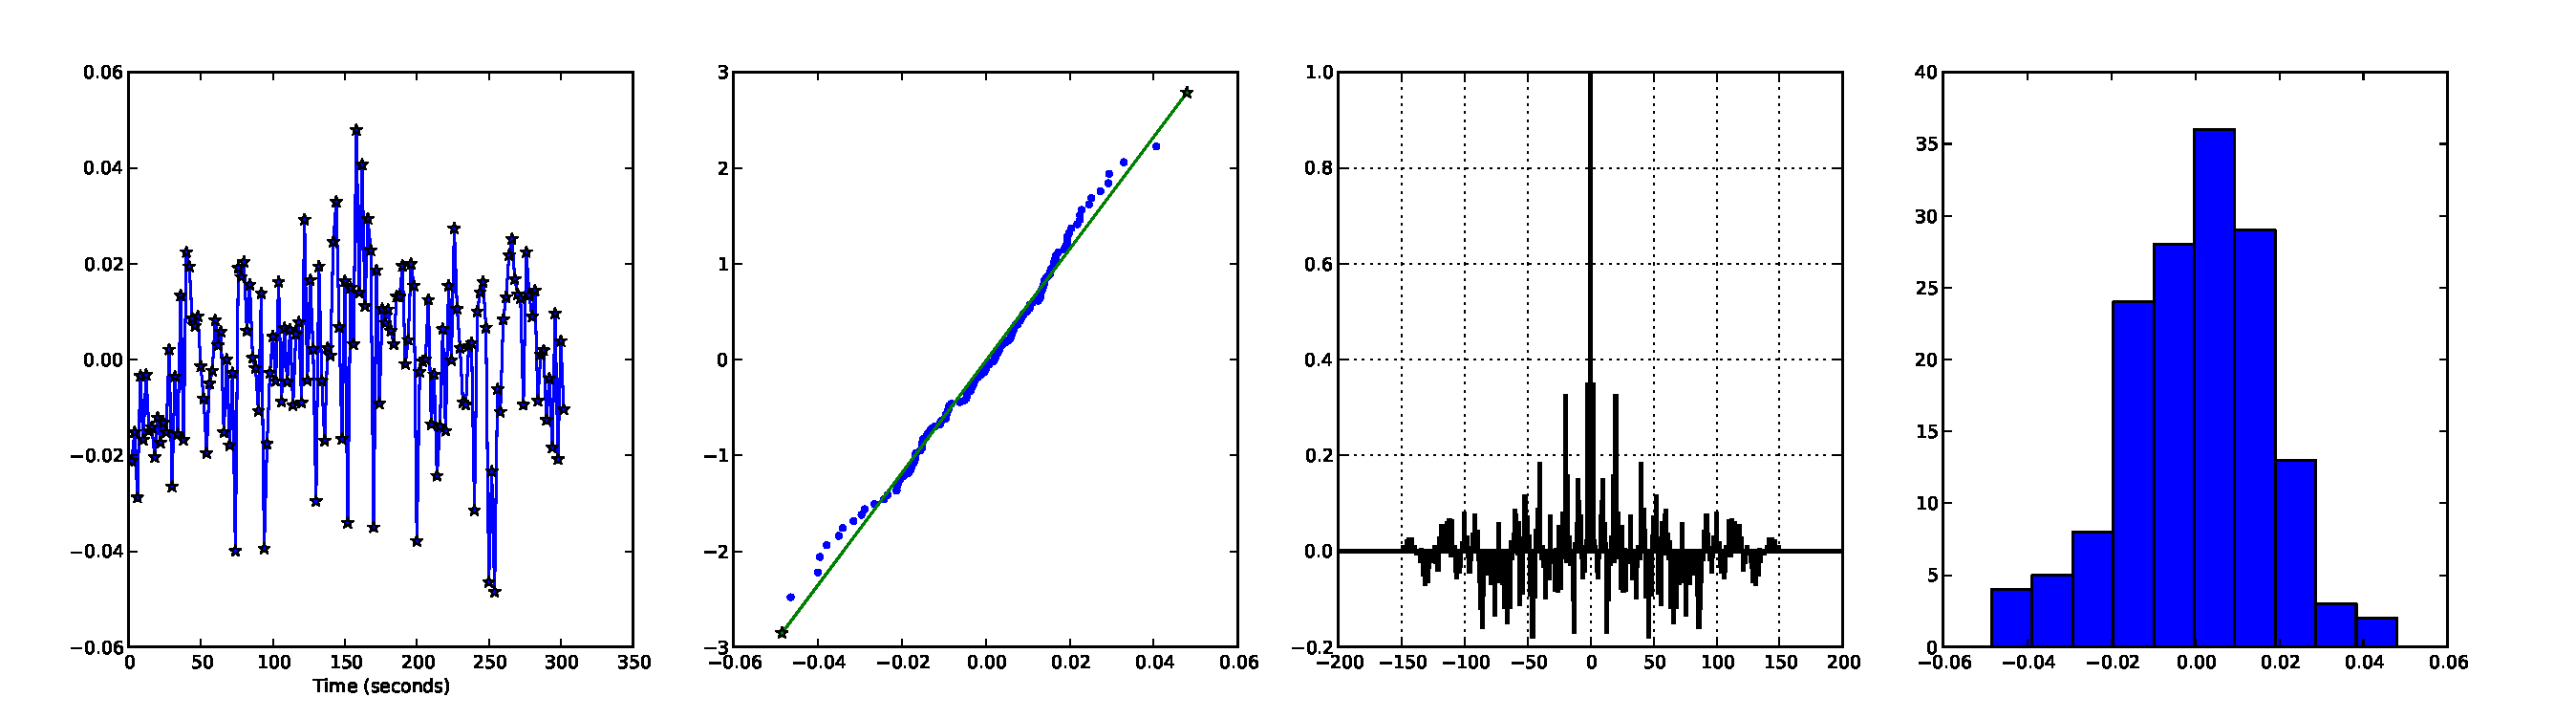
\includegraphics[trim=6cm 1cm 6cm 1cm,width=13cm]{images/noise2_0009_29_49_9}}
\subfigure[]{\label{fig:QQDC:B}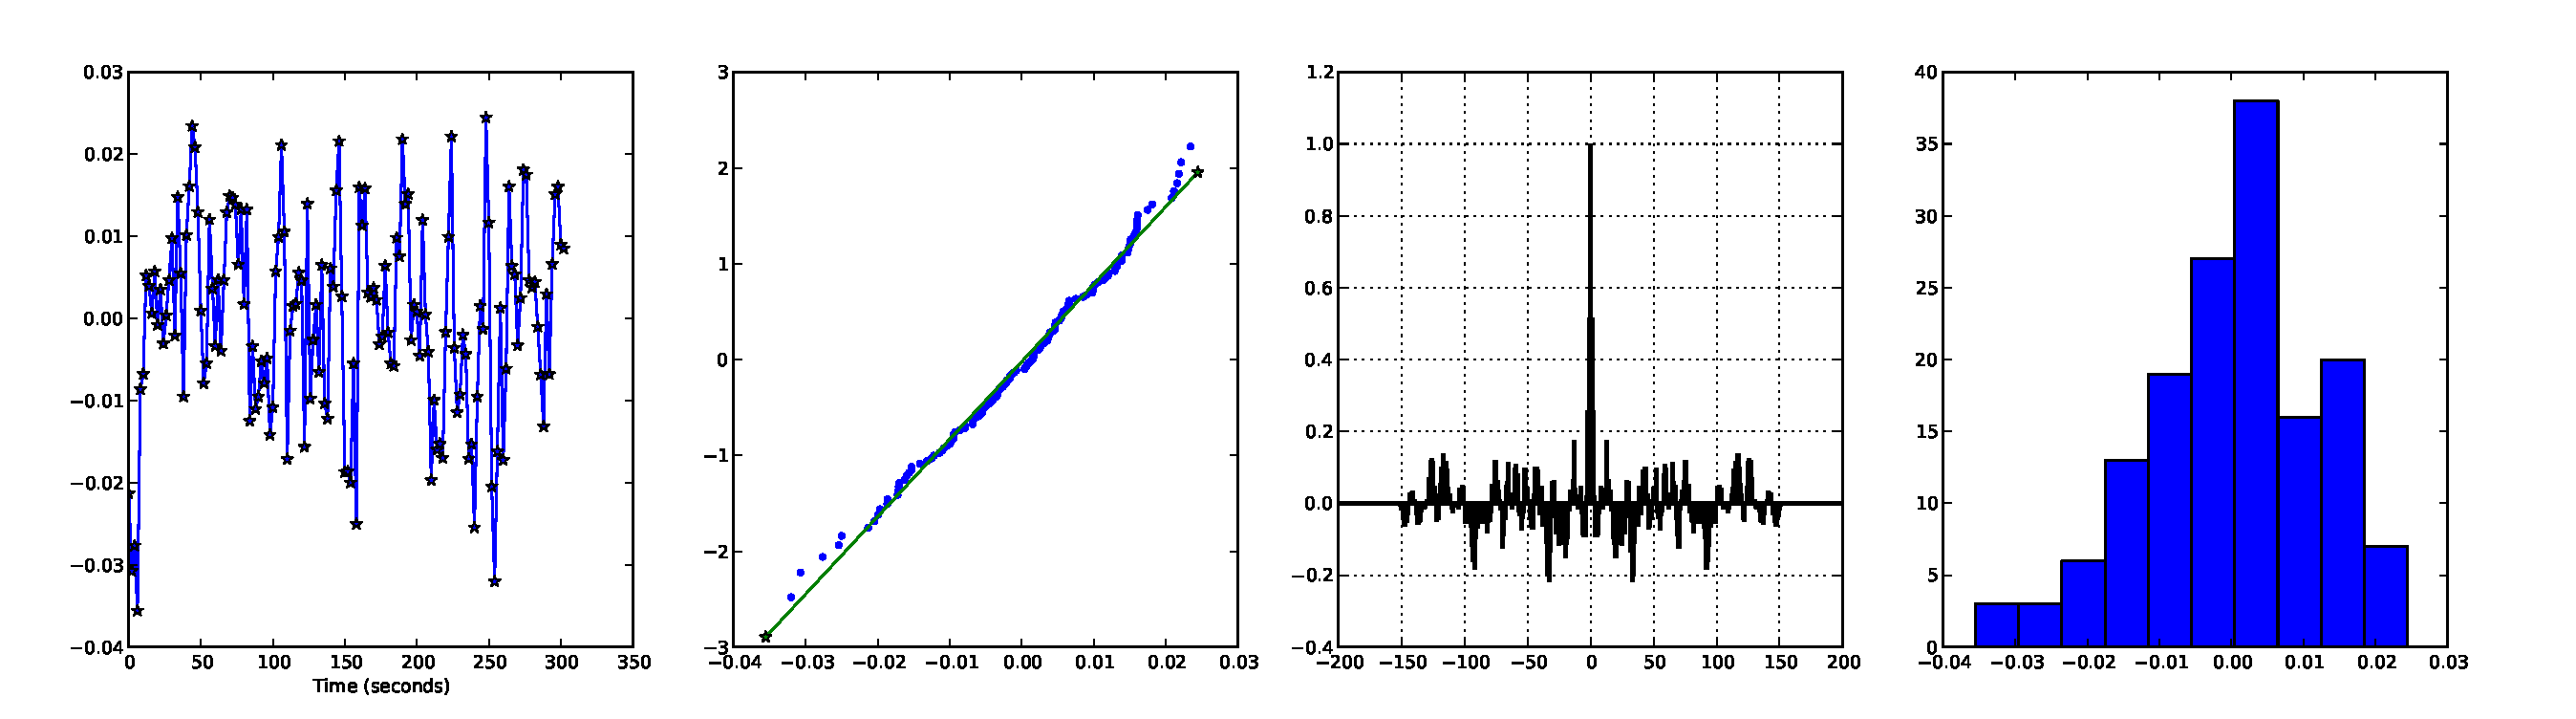
\includegraphics[trim=6cm 1cm 6cm 1cm,width=13cm]{images/noise2_0009_34_43_24}}
\subfigure[]{\label{fig:QQDC:C}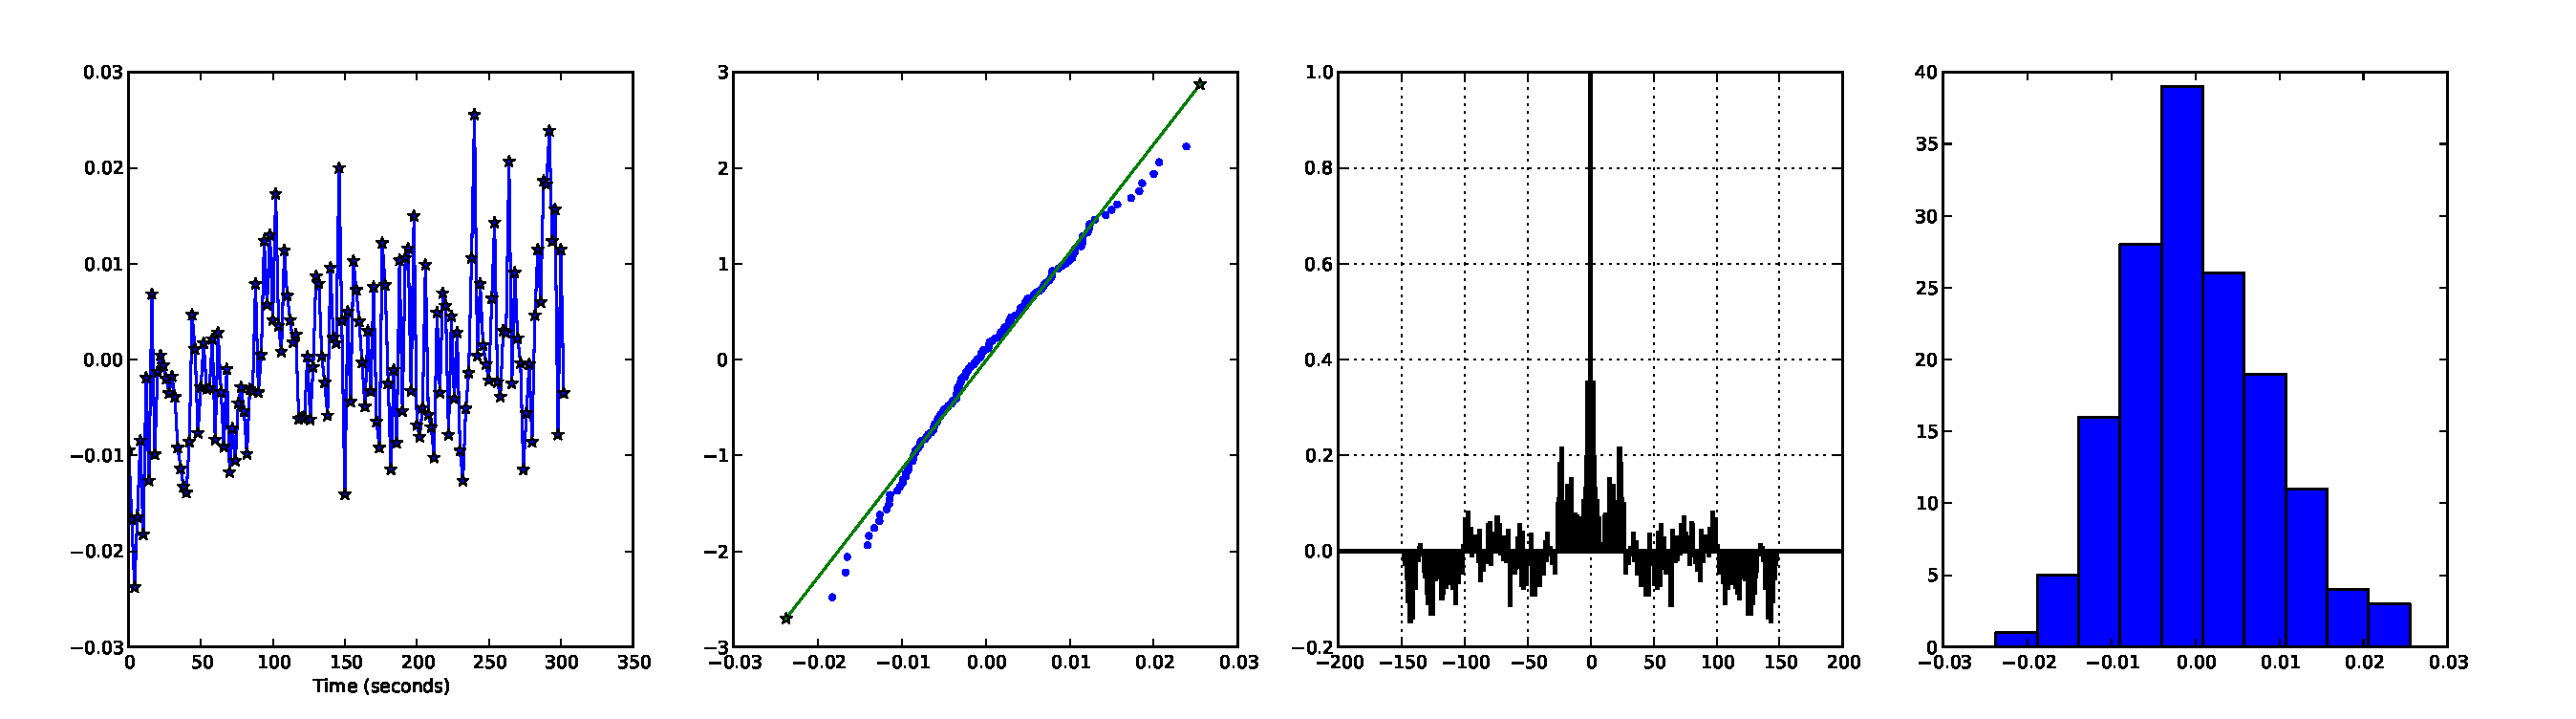
\includegraphics[trim=6cm 1cm 6cm 1cm,width=13cm]{images/noise2_0009_22_38_23}}
\subfigure[]{\label{fig:QQDC:D}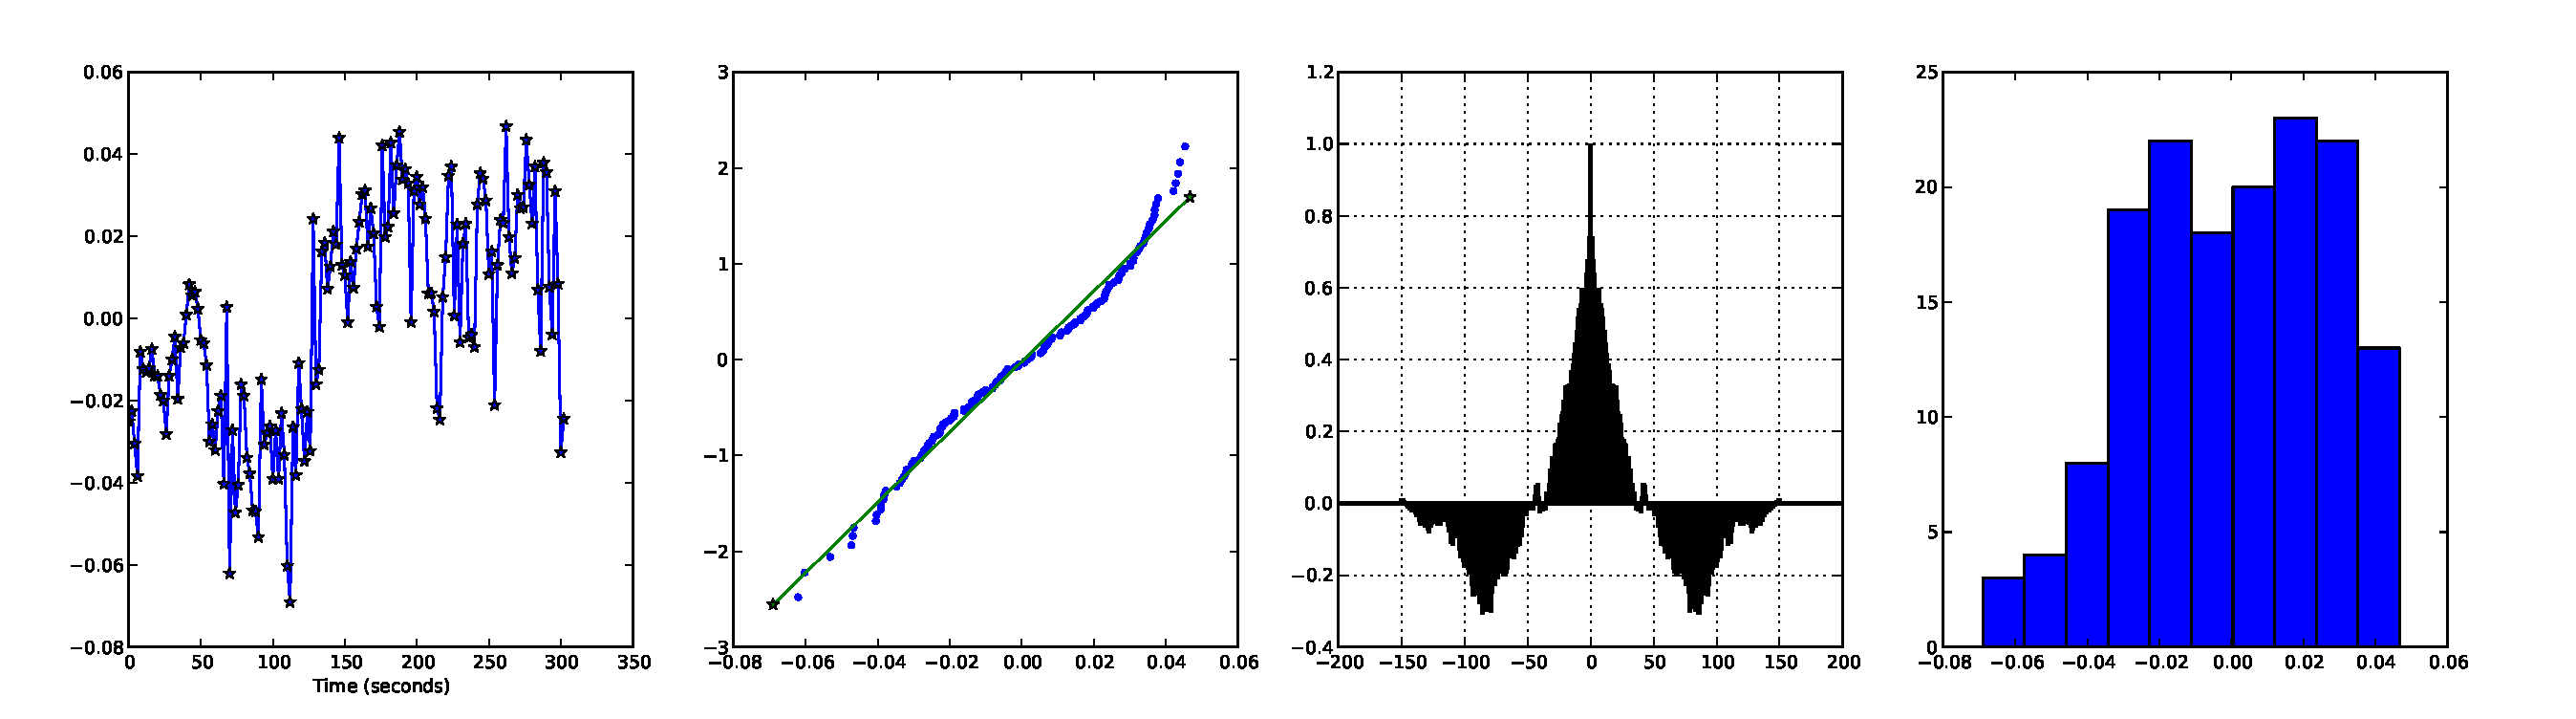
\includegraphics[trim=6cm 1cm 6cm 1cm,width=13cm]{images/noise2_0009_37_29_24}}

%\subfigure{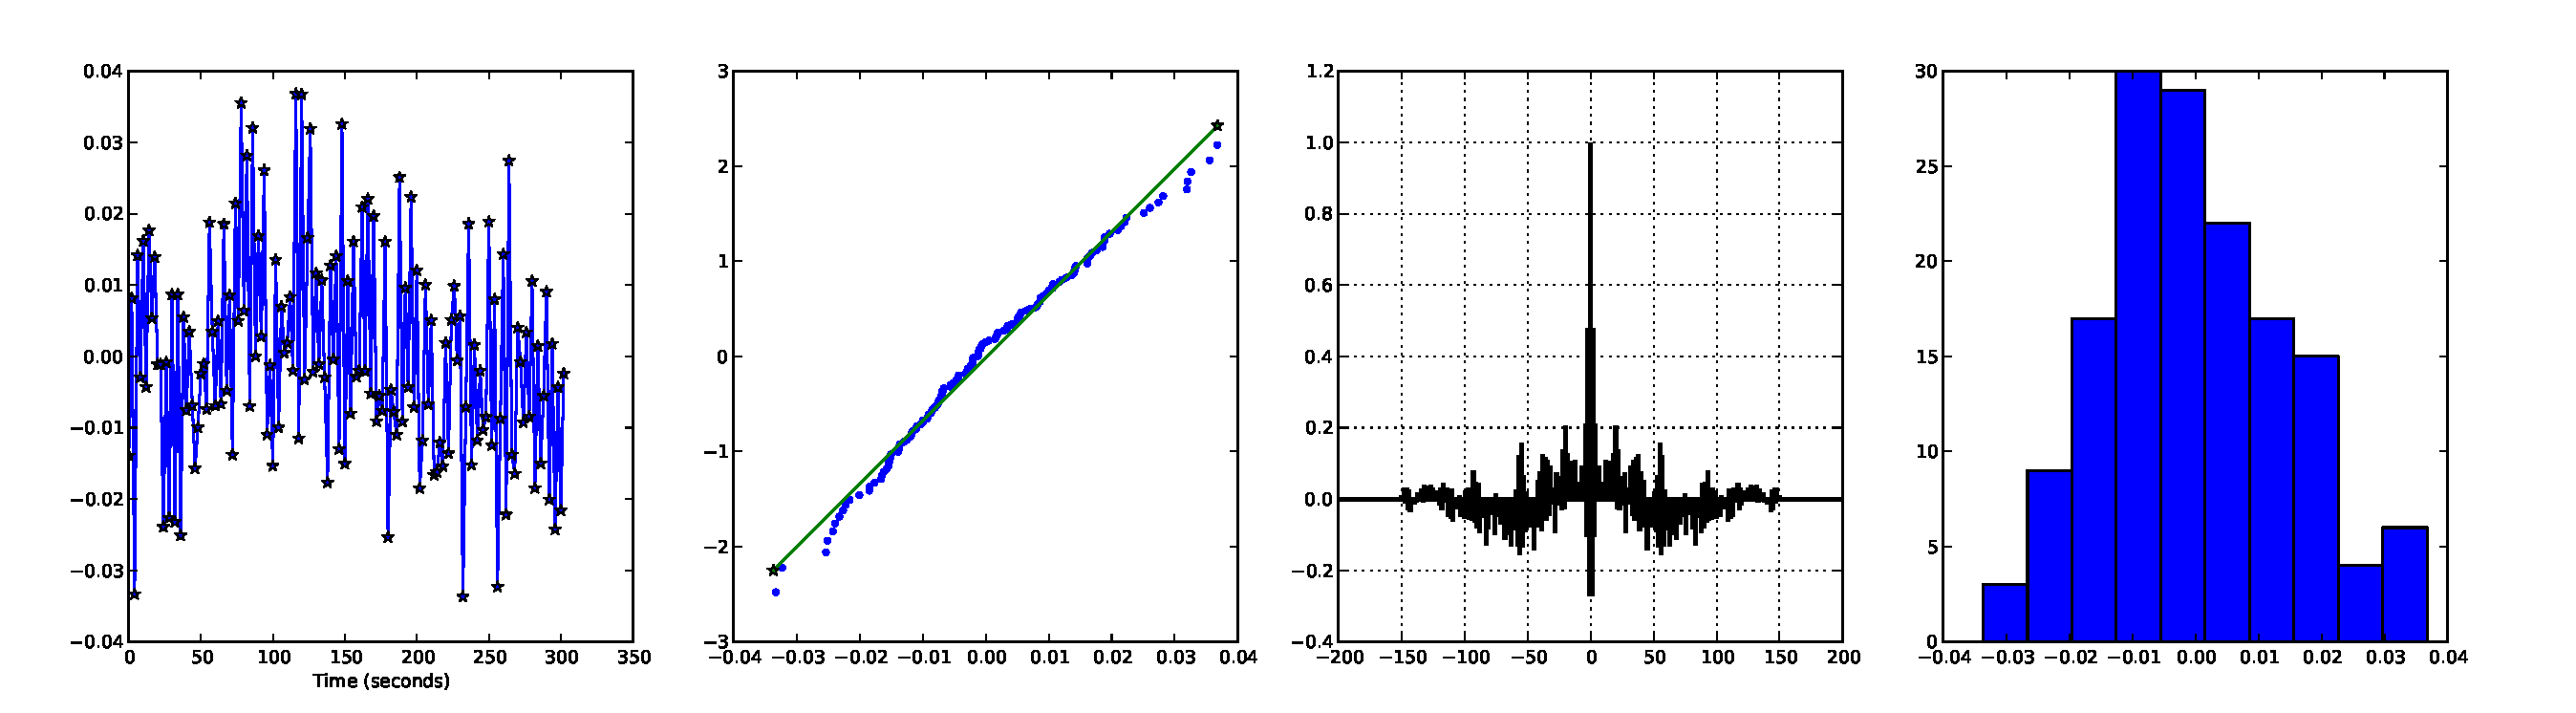
\includegraphics[trim=6cm 1cm 0 0cm,width=17cm]{images/noise_0009_19-24-10.pdf}}
%\subfigure{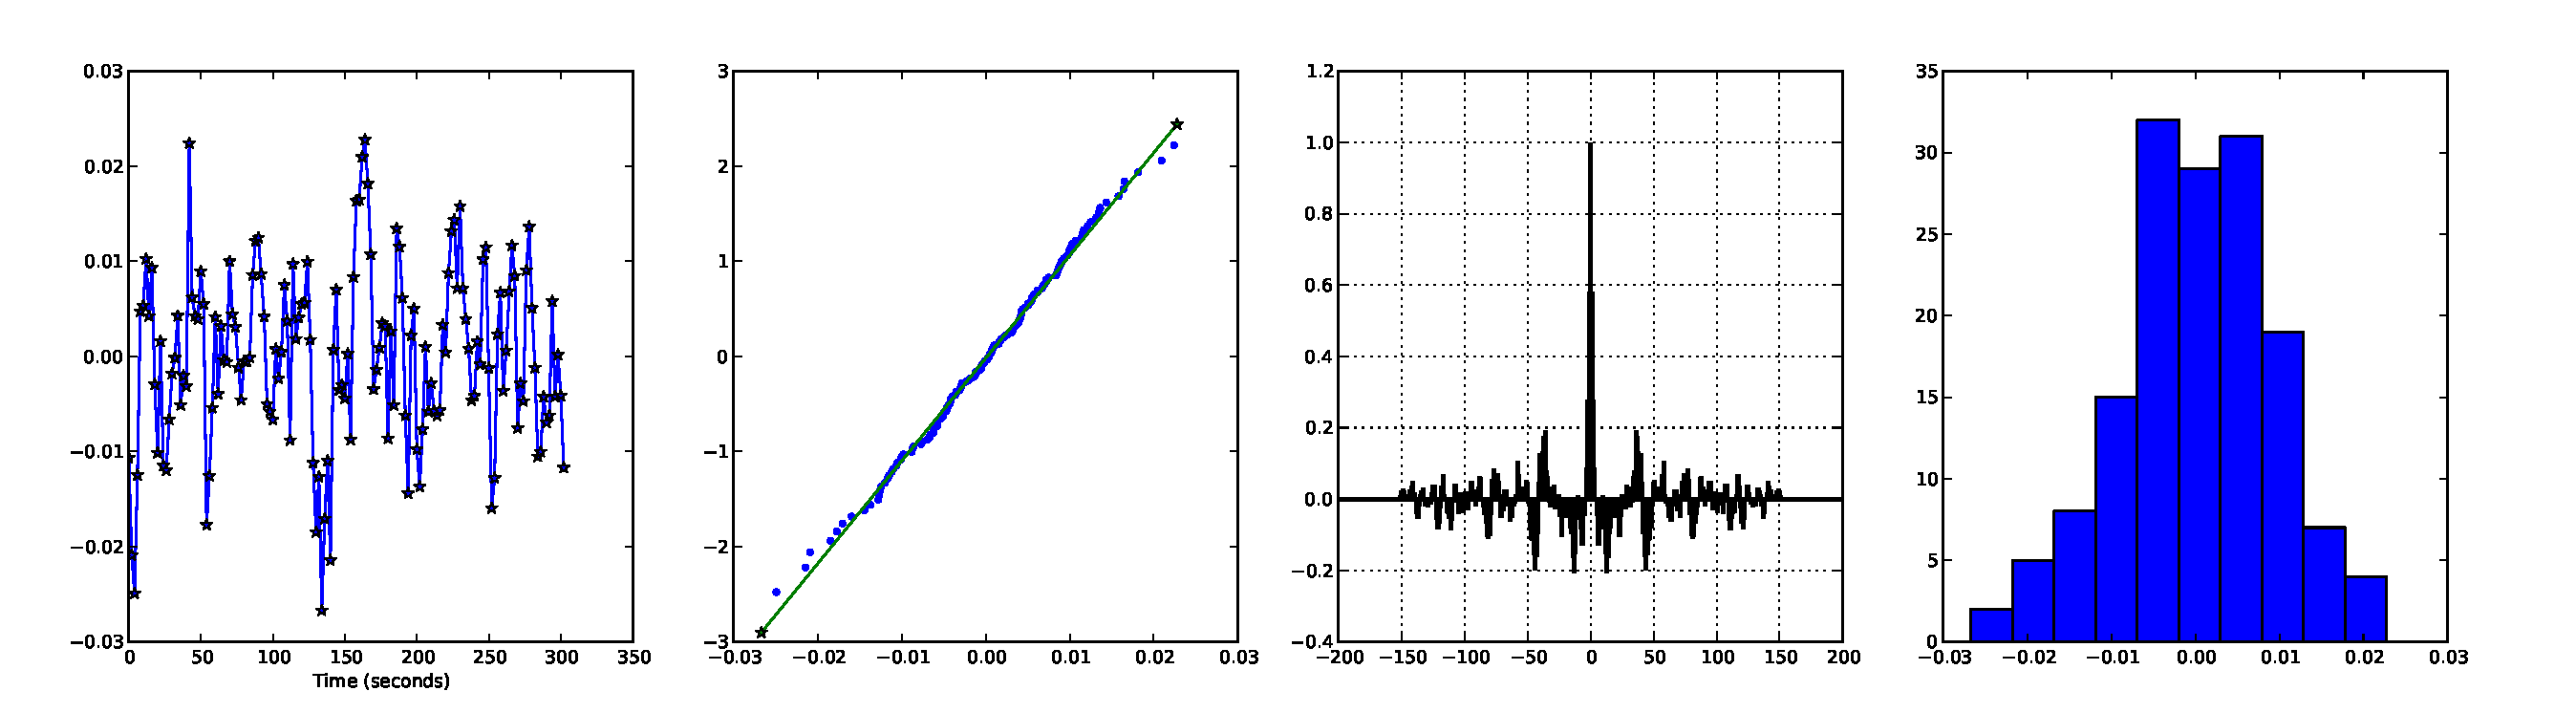
\includegraphics[trim=6cm 1cm 0 0cm,width=17cm]{images/noise_0009_20-45-18.pdf}}
%\subfigure{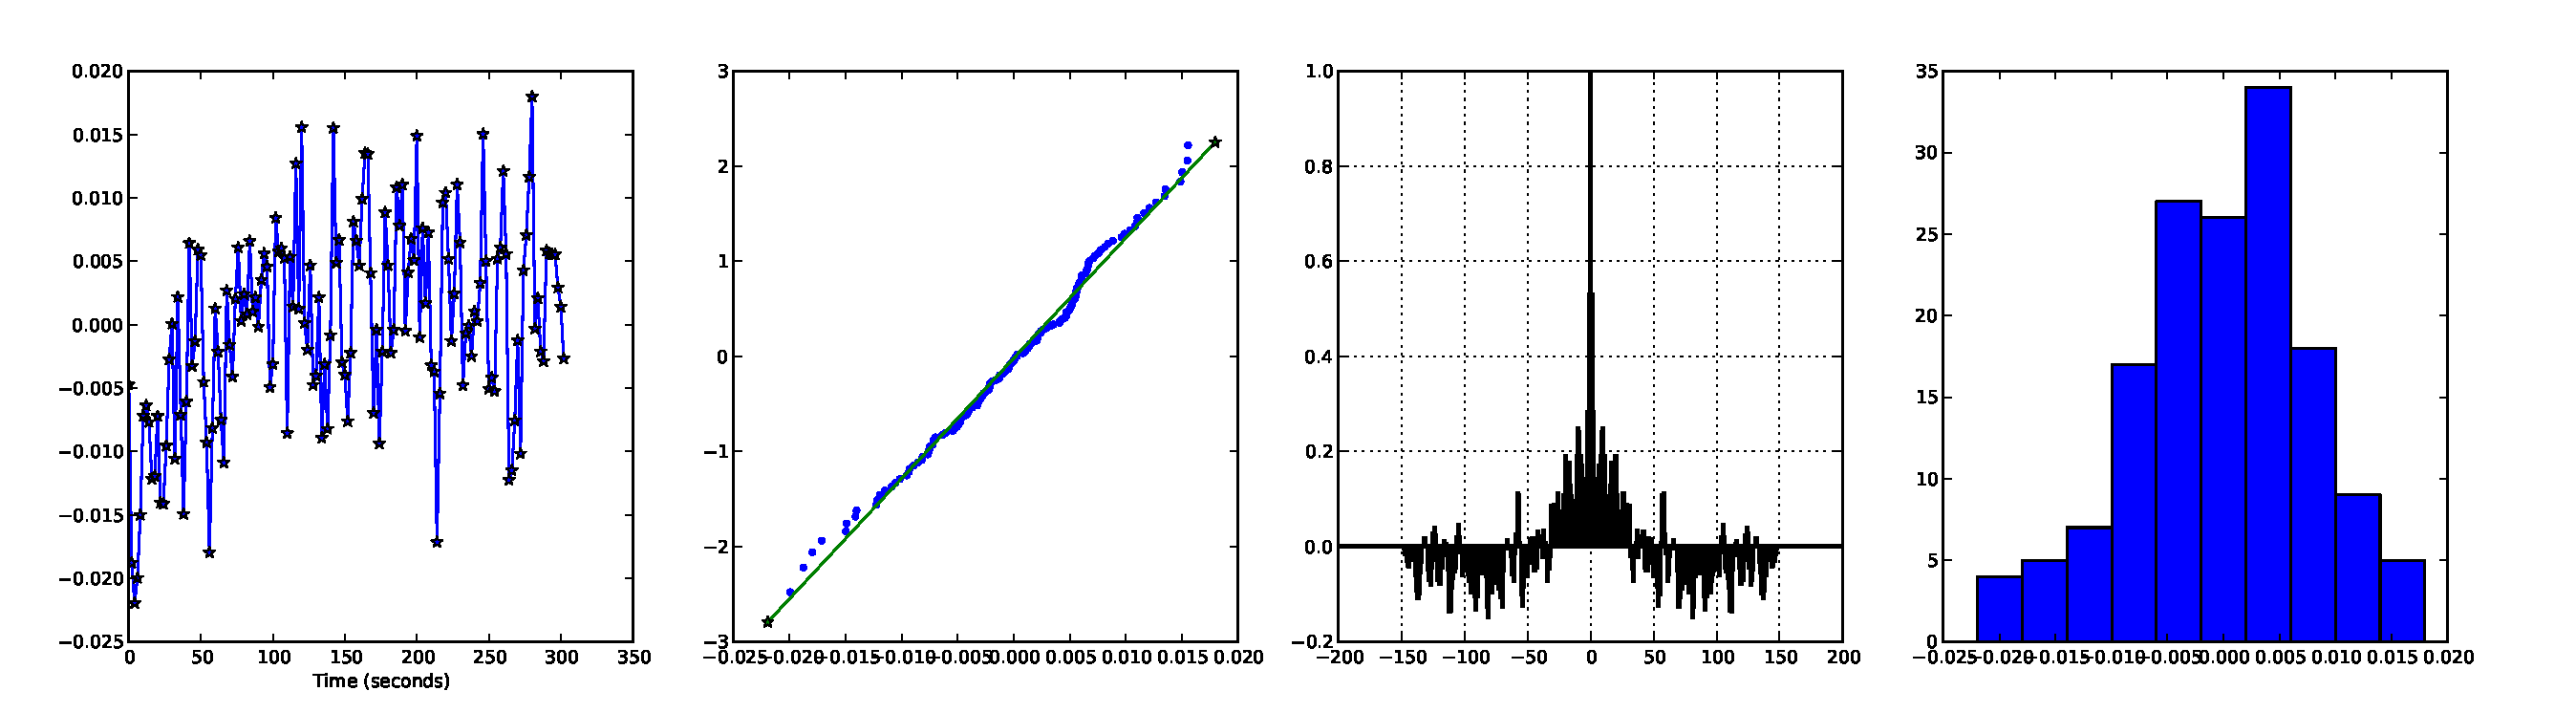
\includegraphics[trim=6cm 1cm 0 0cm,width=17cm]{images/noise_0009_23-47-18.pdf}}
%\subfigure{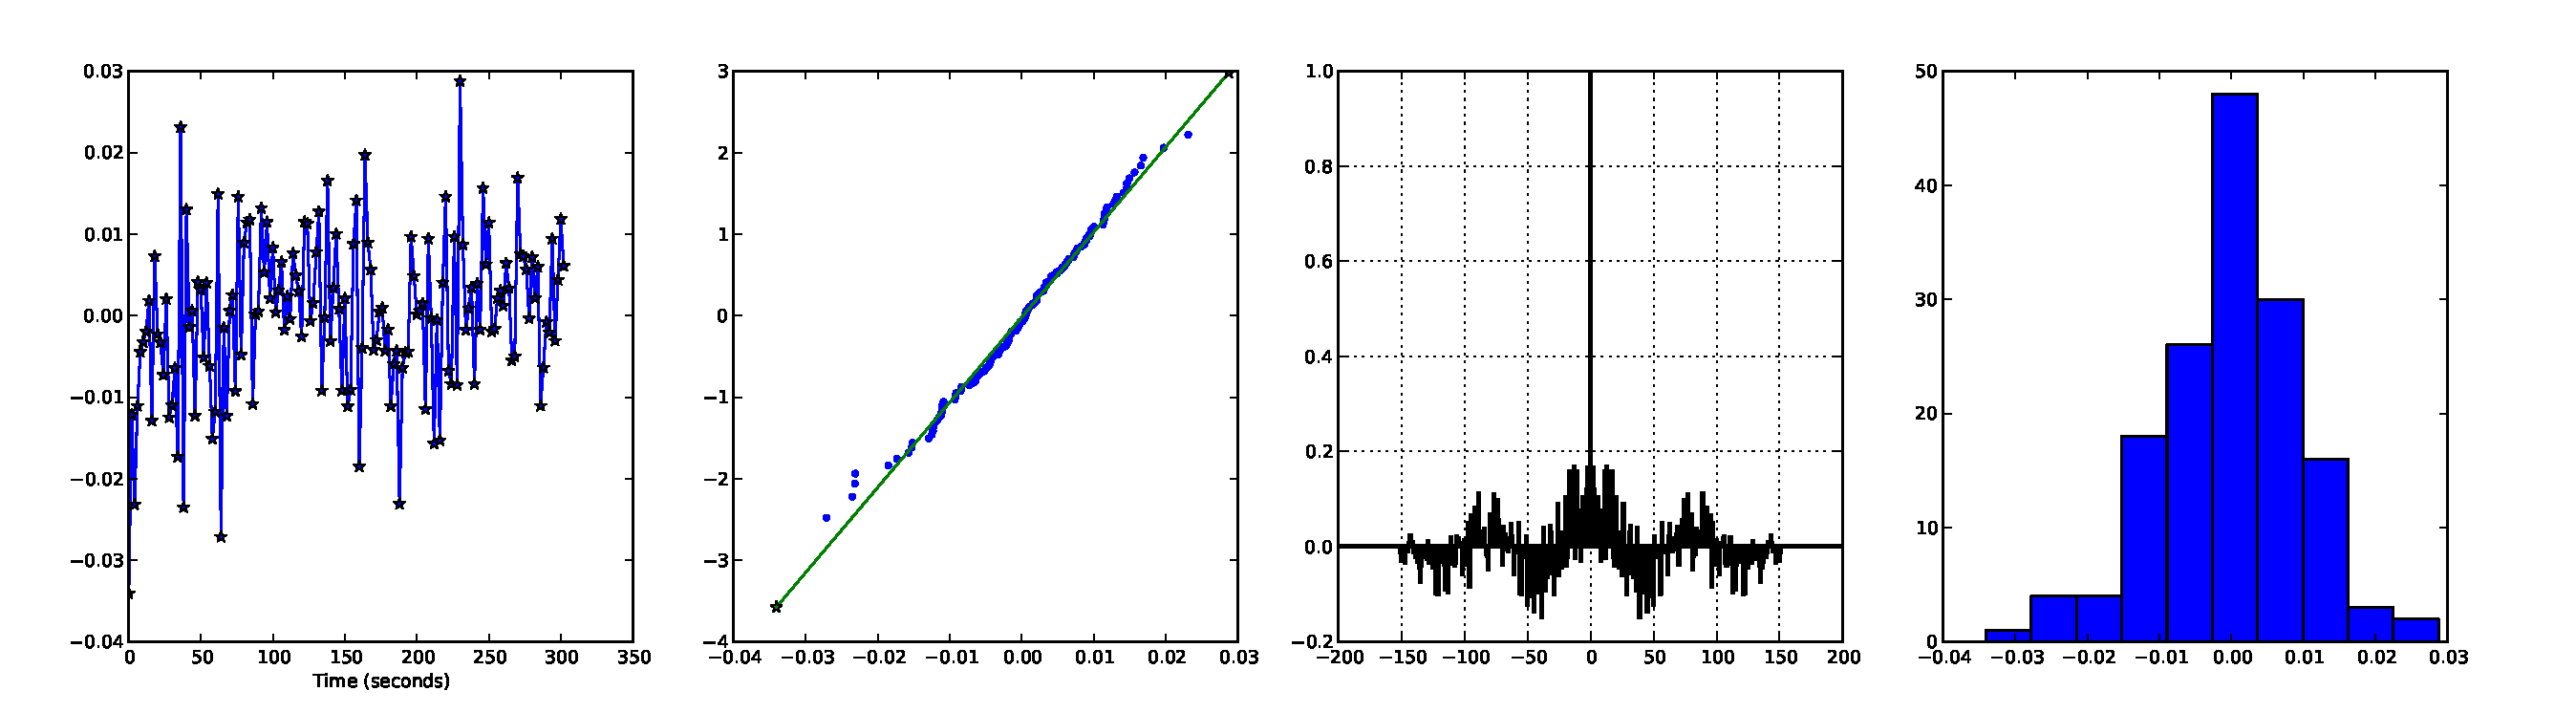
\includegraphics[trim=6cm 1cm 0 0cm,width=17cm]{images/noise_0009_35-49-9.pdf}}

\caption{Q-Q Plots of normalized resting state data}
\label{fig:QQDC}
\end{figure}

\begin{figure}
\centering
\subfigure[]{\label{fig:QQDDelta:A}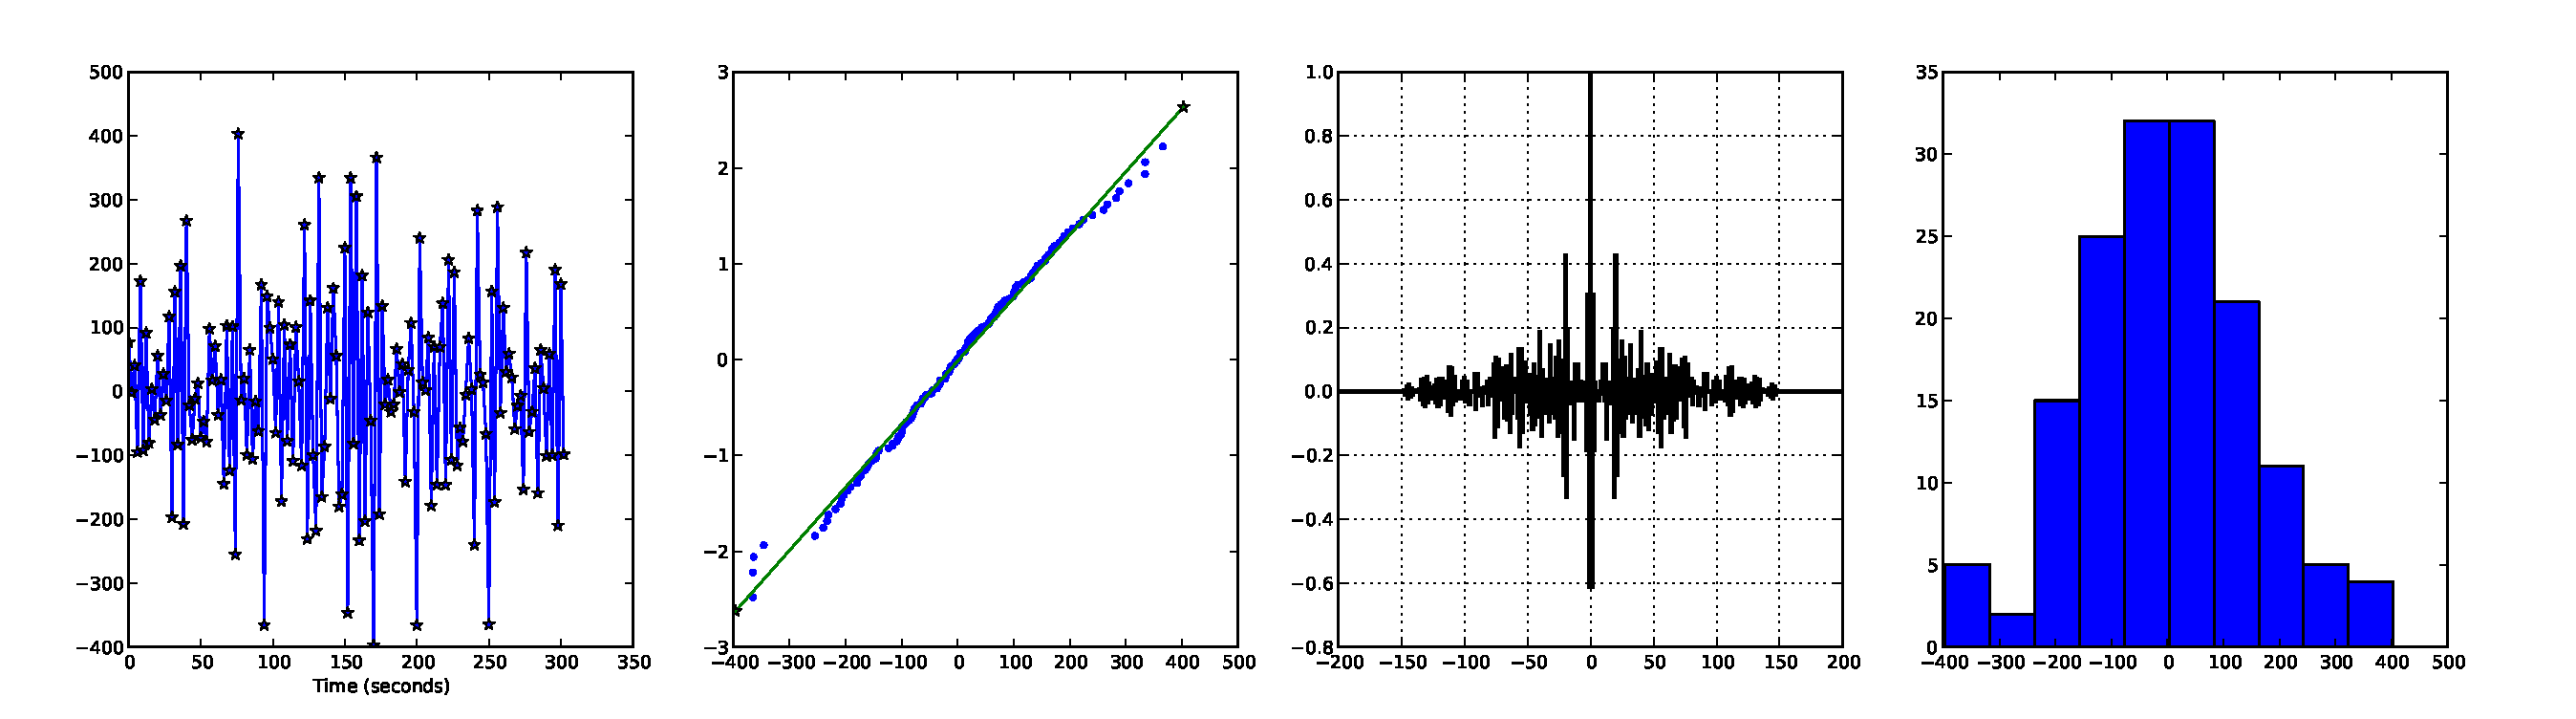
\includegraphics[trim=6cm 1cm 6cm 1cm,width=13cm]{images/noise2_0009d_29_49_9}}
\subfigure[]{\label{fig:QQDDelta:B}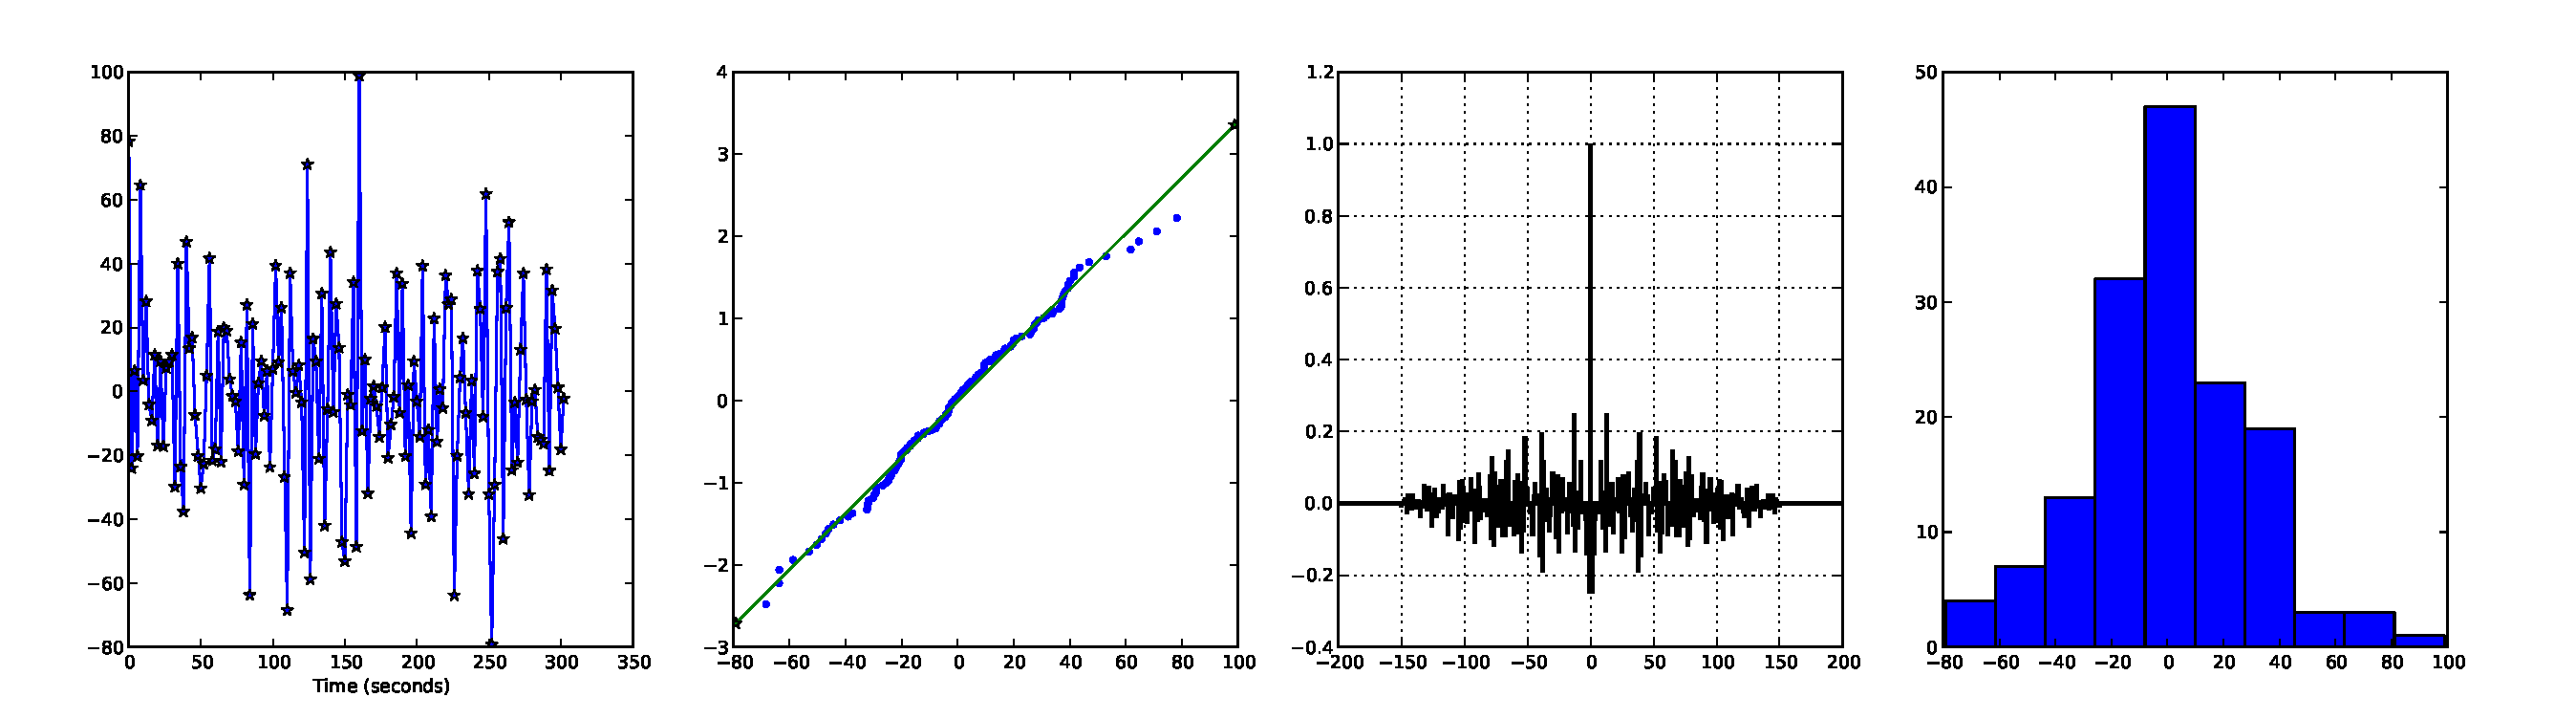
\includegraphics[trim=6cm 1cm 6cm 1cm,width=13cm]{images/noise2_0009d_34_43_24}}
\subfigure[]{\label{fig:QQDDelta:C}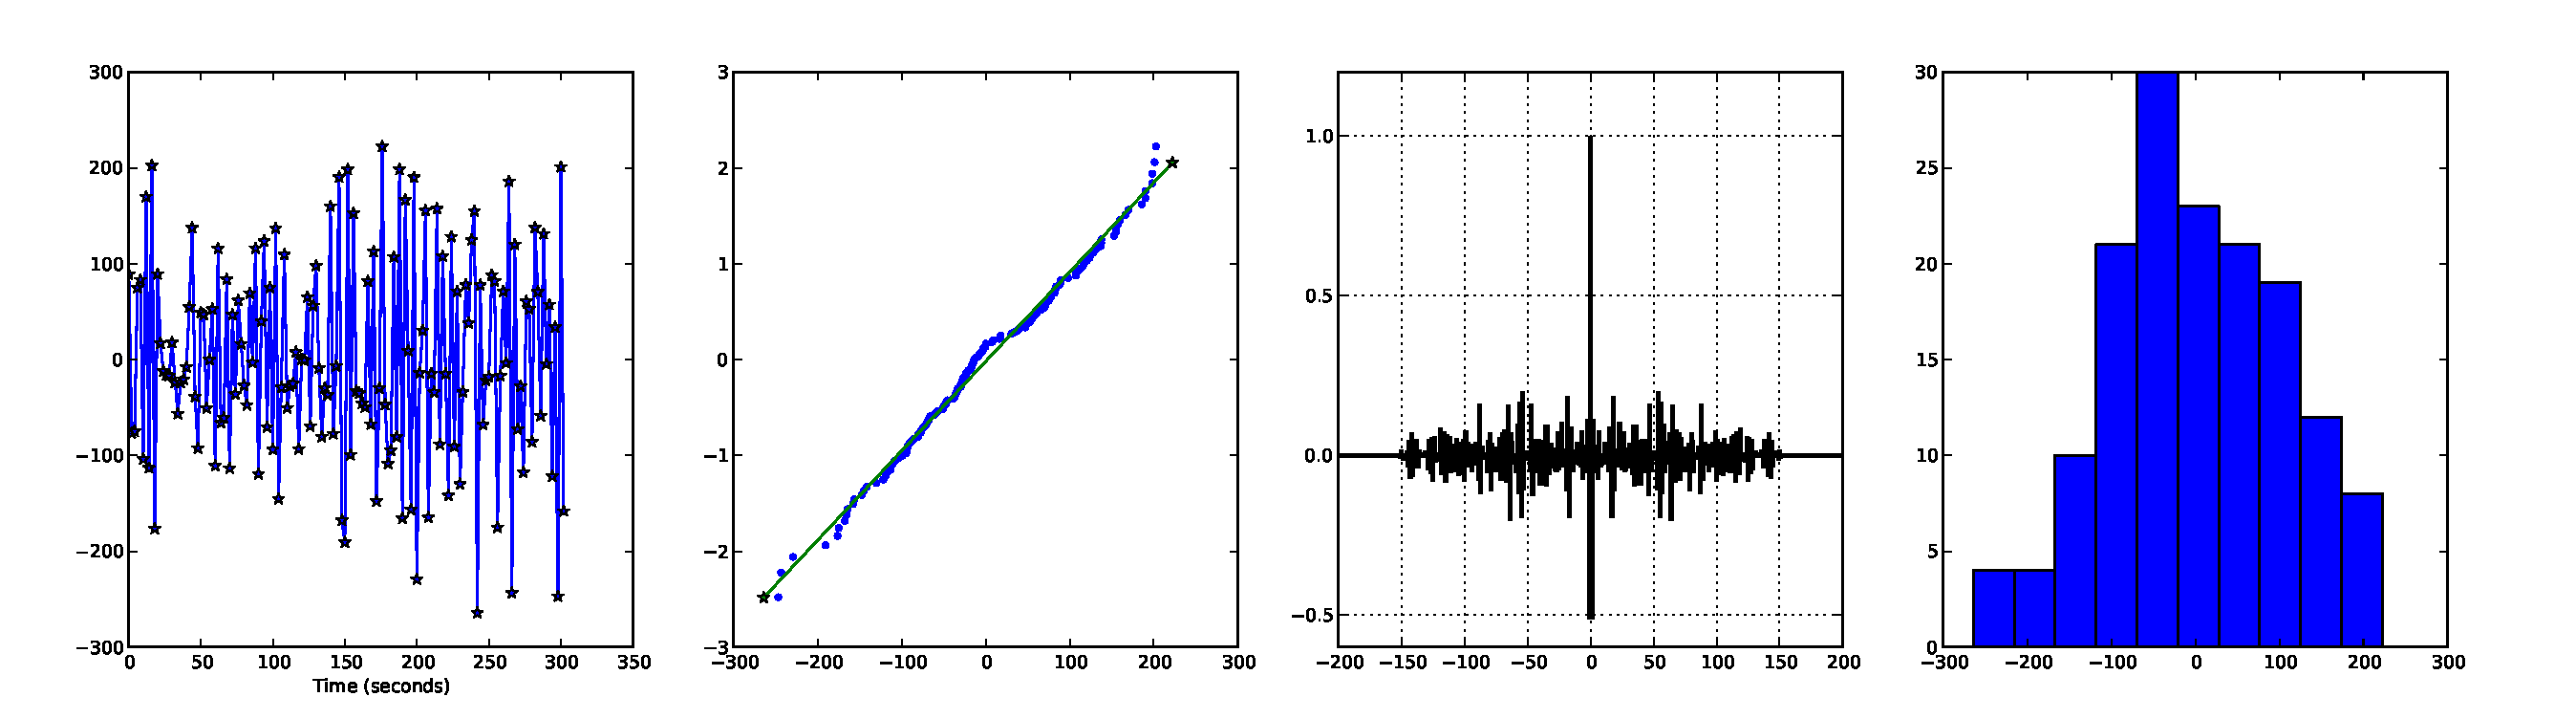
\includegraphics[trim=6cm 1cm 6cm 1cm,width=13cm]{images/noise2_0009d_22_38_23}}
\subfigure[]{\label{fig:QQDDelta:D}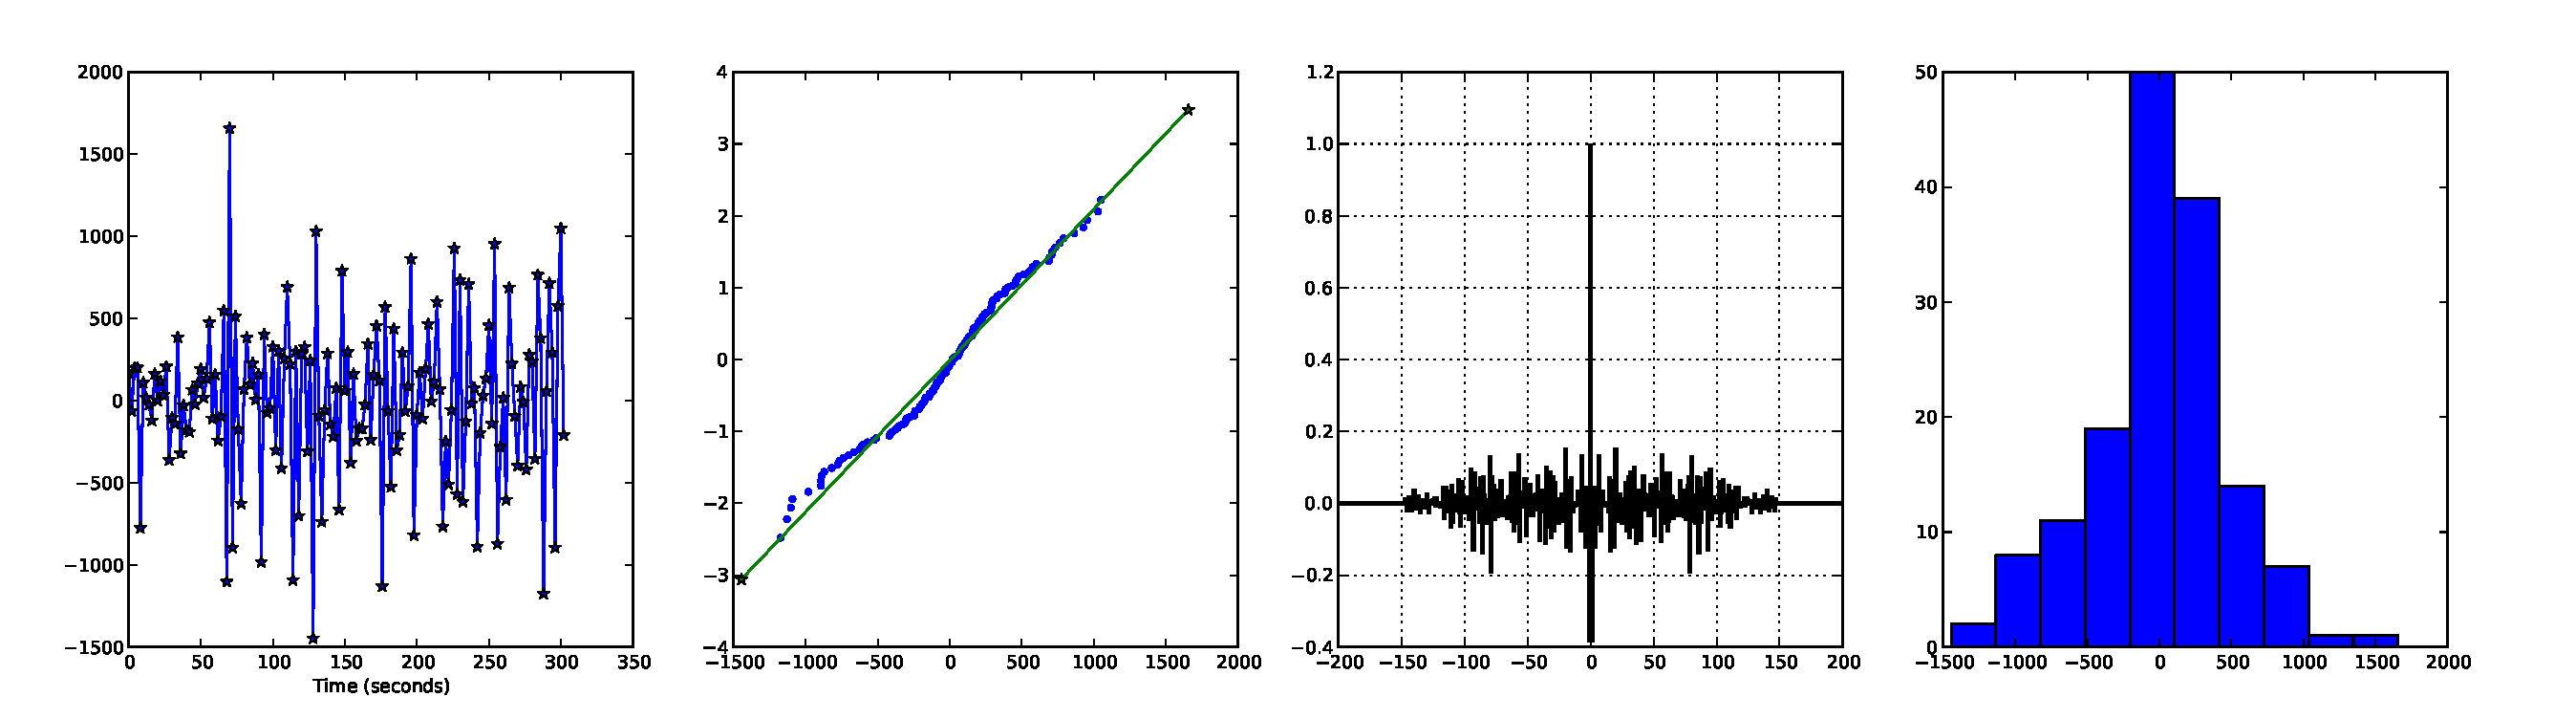
\includegraphics[trim=6cm 1cm 6cm 1cm,width=13cm]{images/noise2_0009d_37_29_24}}
\caption{Q-Q Plots of resting state data, using the BOLD signal changes}
\label{fig:QQDelta}
\end{figure}

A Wiener process should still conform to the normal distribution, with a 
variance proportional to the run-time. Note that \autoref{fig:QQDC:A} and \autoref{fig:QQDC:B}
are well described by a Gaussian process with a small autocorrelation, 
\autoref{fig:QQDC:C} and \autoref{fig:QQDC:D} are not. In particular the tails of \autoref{fig:QQDC:C}
do not seem to fit the Gaussian well. Also note the significant autocorrelation in
\autoref{fig:QQDC:C} and \autoref{fig:QQDC:D}. As expected, the noise is not strictly
Gaussian white noise.  On the other hand, the steps do conform rather
closely to the normal distribution.
As expected, most of the autocorrelation disappears for the step data. Given
that the steps seem to fit the Normal distribution, the low autocorrelation
indicates that the steps could be Independently Distributed. 
Therefore, the noise does come close to a Wiener process. 

\begin{figure}
\centering
\subfigure[]{\label{fig:QQs:A}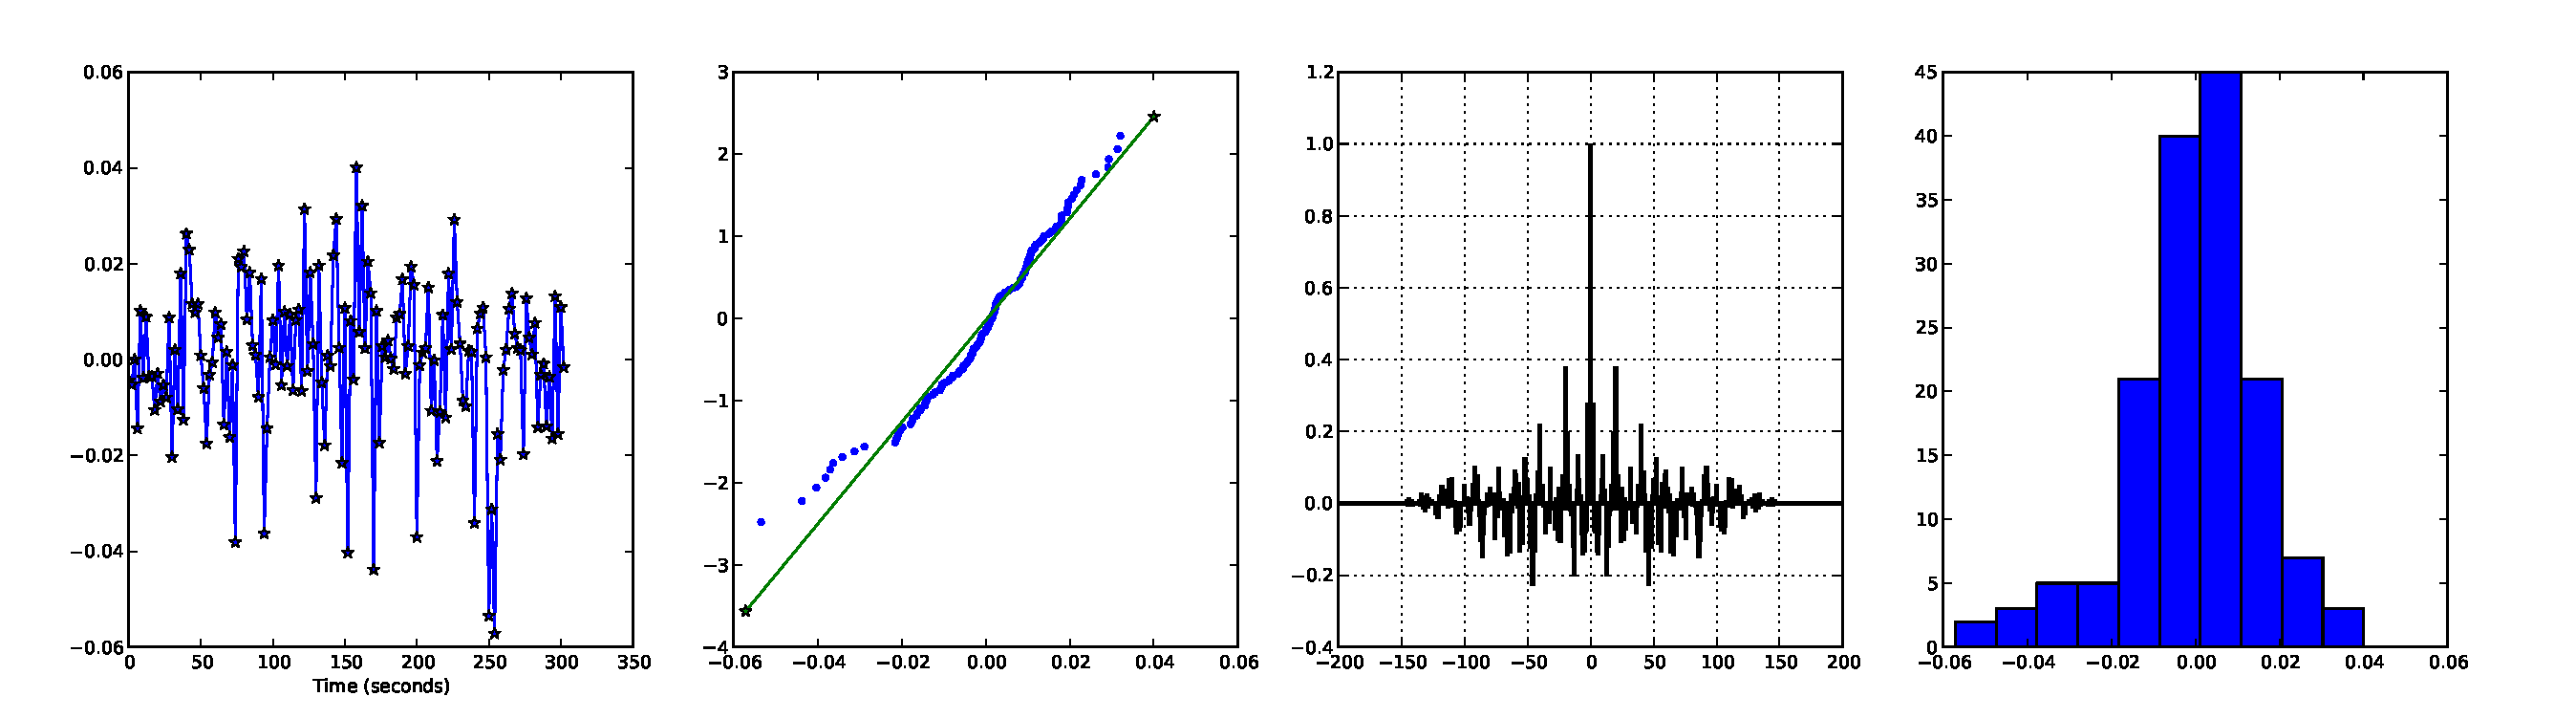
\includegraphics[trim=6cm 1cm 6cm 1cm,width=13cm]{images/noise2_0009s_29_49_9}}
\subfigure[]{\label{fig:QQs:B}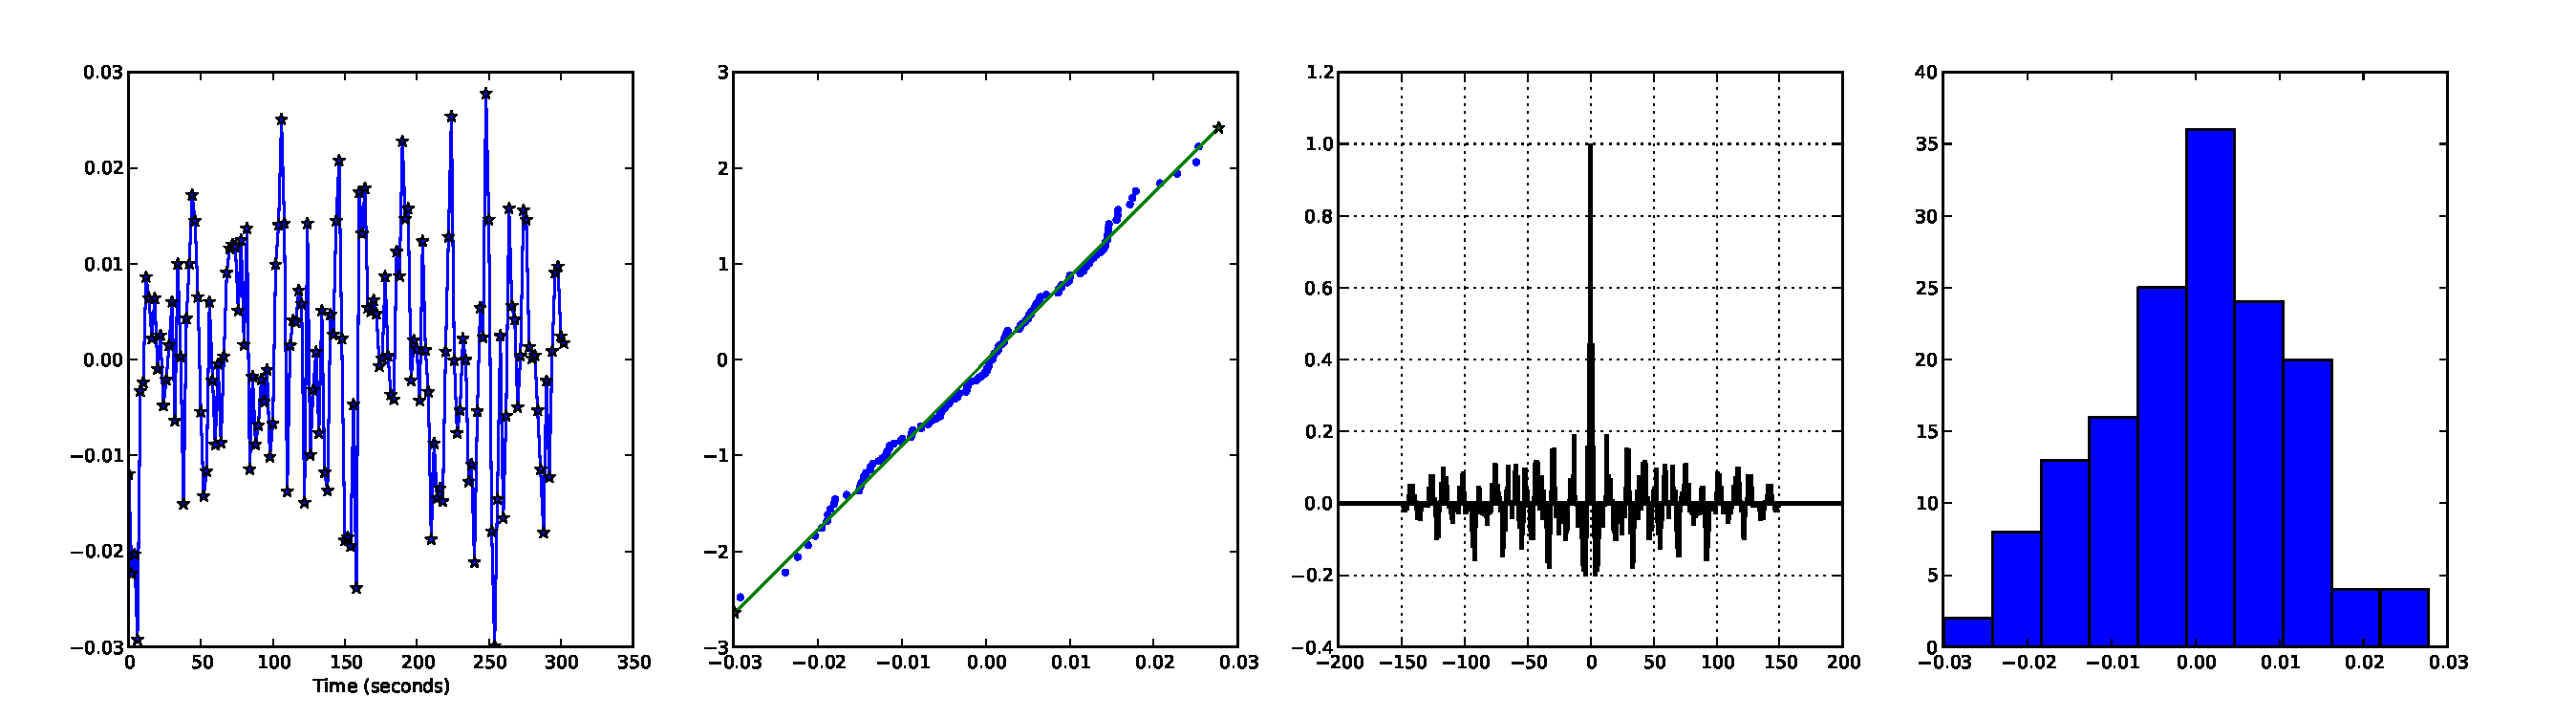
\includegraphics[trim=6cm 1cm 6cm 1cm,width=13cm]{images/noise2_0009s_34_43_24}}
\subfigure[]{\label{fig:QQs:C}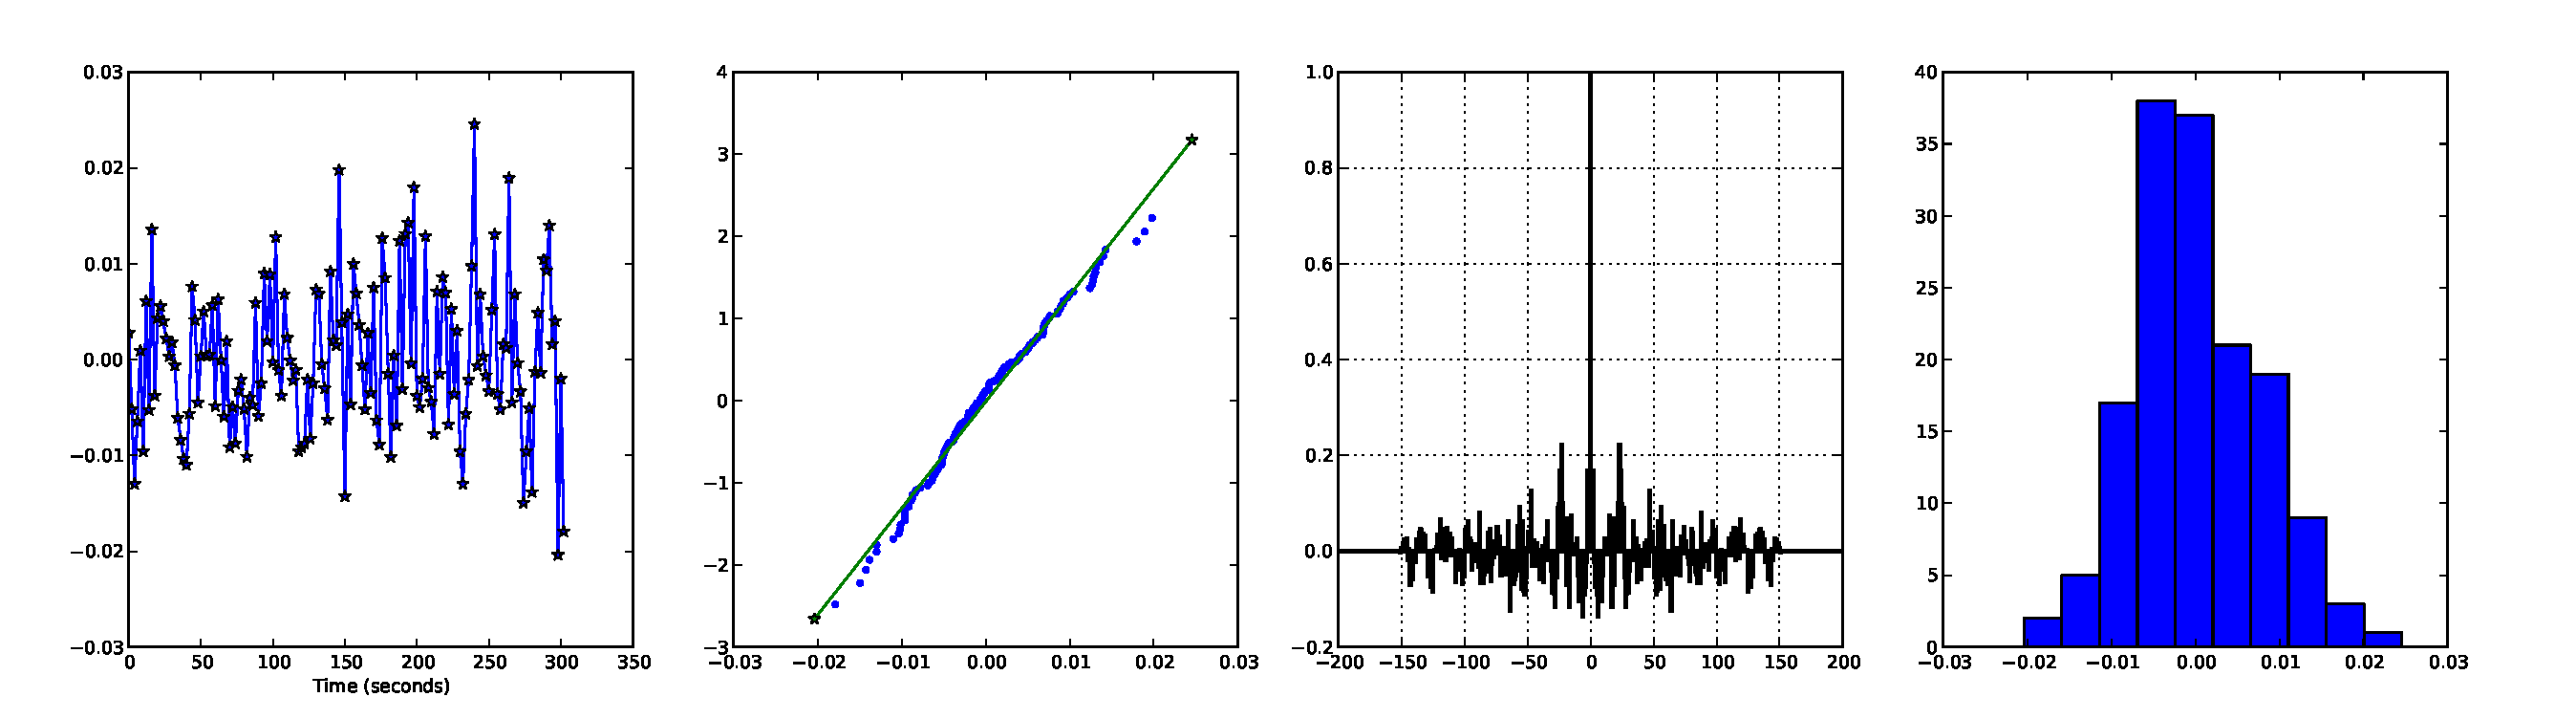
\includegraphics[trim=6cm 1cm 6cm 1cm,width=13cm]{images/noise2_0009s_22_38_23}}
\subfigure[]{\label{fig:QQs:D}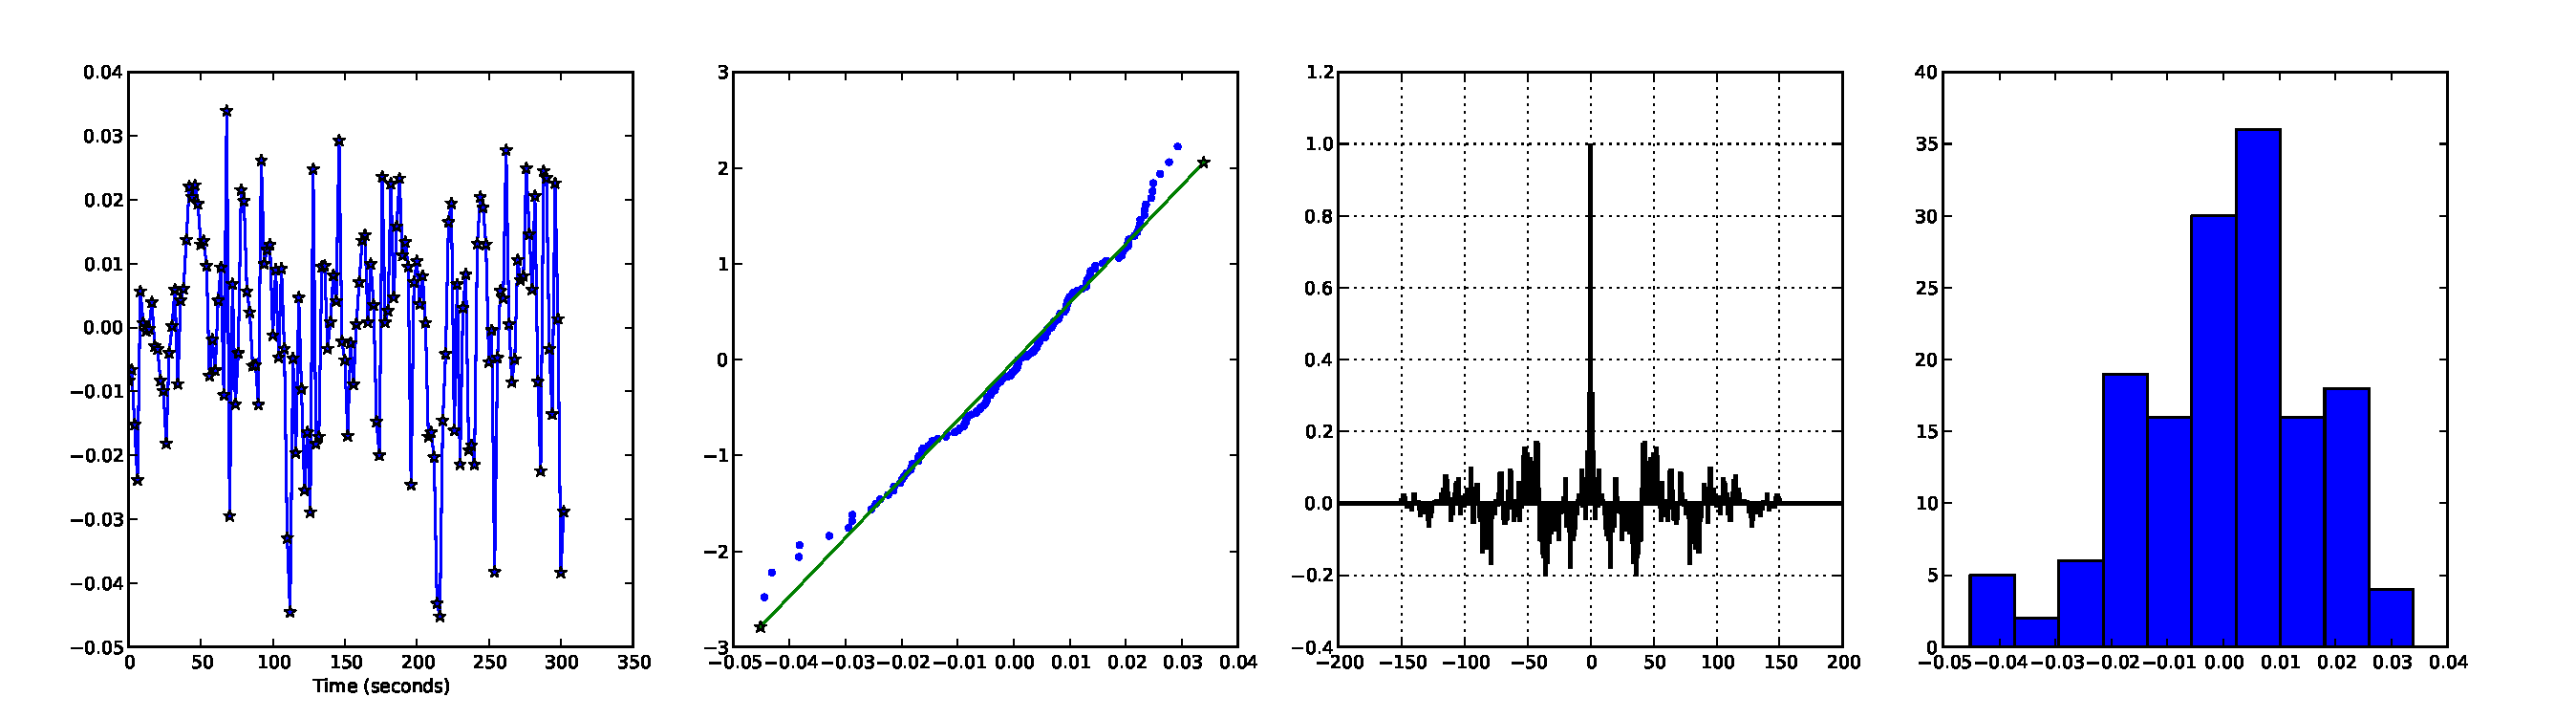
\includegraphics[trim=6cm 1cm 6cm 1cm,width=13cm]{images/noise2_0009s_37_29_24}}
\caption{Q-Q Plots of resting state data, after the de-trending}
\label{fig:QQSpline}
\end{figure}

De-trending the time-series by subtracting a spline fit to the distribution
removed much of the autocorrelation present in \autoref{fig:QQDC:C} and \autoref{fig:QQDC:D},
though not perfectly. Though the distributions still do not exactly fit
the Normal, \autoref{fig:QQs:D} is much improved compared to \autoref{fig:QQDC:D}.
In all, the de-trending is effectively removing Wiener noise. 

\subsection{Detrending}
\label{sec:Detrend}
The non-stationary
aspect of a Weiner process, presumably the result of integrating some
$\nu_x$ is difficult to compensate for, and so methods
have been developed to compensate for it. \cite{Tanabe2002} and \cite{Smith1999} have
demonstrated that this component is prevalent, and may in fact be an inherent  characteristic
of FMRI. In some studies, as many as half the voxels benefit from detrending, presenting
a serious barrier to inference (\cite{Smith2007}). All the existing methods are performed
during the preprocessing stage, rather than as an integral part of analyzing the BOLD
signal. There is no shortage of detrending methods; however
in a head to head comparison, \cite{Tanabe2002}, showed that in most cases subtracting off
a spline works the best. The benefit of the spline versus wavelets, high pass 
filtering or other DC removal techniques is that the frequency response is not set.
Rather, the spline is adaptive to the input, having a low cut off if the signal's 
median stays constant but a high cut off frequency if the signal's median tends to
shift heavily over the course of time. In spite of this, the spline will still remove some
amount of signal.

The method I used to calculate the spline was picking one knot for every 20
measurements in an image. Thus a 10 minute session at a repetition time of 
2.1 seconds would have 19 knots. The knot first and last knots were each 
given half the number of samples as the rest of the knots; which were all 
located at the center of their sample group. The median of each sample group
was then taken and used as the magnitude for the group. Taking the median 
versus the mean seemed to work better, given the presence of outliers. 
There is potential to optimize the spline further using a canonical 
HRF to find resting points; however, for this to work the experiment would have
to be designed with this in mind. 

When using the median-based spline techniques, the normalized signal will,
by definition have a median near zero. 
The problem with this is this is not the natural state of the BOLD signal. More specifically,
when the signal is inactive, the BOLD response should be at 0\% change from
the base level; activation may then increase, or for short periods decrease from this base.
After removing the spline, the BOLD resting state will be below 0\%.
This is problematic because it reduces the ability of an algorithm to learn.
One quick and dirty solution is to add an arbitrary constant to each BOLD response. 
Of course this won't scale to whole-brain analysis, so a more effective technique 
is adding a DC gain parameter to the BOLD model. 
Like all the other model parameters, given enough measurements, correct
value may be found. On the downside, adding another dimension increases the
complexity of the model, for a variable that is obvious by direct
observation.

Thus, I used a more conventional approach to deal with this. To determine
the DC gain to be added to the signal I used a robust estimator 
of scale. The Median Absolute Deviation (MAD)
proved to be accurate in determining how much to shift the signal up
by. I tested both methods during the course of analysis, and found that the increase 
in model complexity far outweighed the slight increase in flexibility. Its 
possible that a more accurate method may exist; however, for this case the 
MAD works well, as \autoref{fig:PreprocessedLowNoise} and \autoref{fig:PreprocessedHighNoise} show. 

\begin{equation}
y_{\text{gain}, 0:K} = 2\text{median}_{i=0:K}(y_i - \text{median}(y_{0:K}))
\end{equation}

A serious concern with adding and subtracting arbitrary values to 
real data is whether this will create false positives. This is a legitimate
concern; however, all the additions and subtractions done in this section
have been low frequency changes and should not substantially change
the BOLD response, being a higher frequency signal. The typical
method of preprocessing is a high-pass filter with a cutoff of around 30
seconds; which should about match the spline with knots every fifteen 
measurements. \cite{Tanabe2002} found that splines tended to far outperform the
high-pass filter method. 

%\subsection{Linearizing Noise}
%\label{sec:Methods Delta Based Inference}
%The alternative to these sorts of low frequency manipulation is to
%go around the problem in another way. Here, I propose a 
%different method of dealing with the drift. 
%Instead of comparing the direct output of the particle filter with the direct
%measurement, the algorithm would compare the change in signal over a single TR,
%with the result of integrating the model for the same period. 
%In most signal processing cases this would be foolish, but that is because the 
%general assumption is that all noise is high frequency. Considering 
%the fact that every BOLD analysis pipeline uses a high pass filter,
%whereas low poss temporal filter are rarely applied, it makes sense
%that a derivative type method could work. The benefit of particle filters
%is that they are a robust method of inference, and I would assert 
%that the particle filter ought to be given as \emph{raw} data as possible. 
%While taking direct measurements
%without de-trending would give awful results, using the difference removes the 
%DC component and turns what is usually assumed to be a Weiner process into 
%a simple Gaussian random variable. 
%
%\begin{equation}
%\Delta y = y(t) - y(t-1) = g(x(t)) - g(x(t-1)) + \nu_y(t) - \nu_y(t-1) + \nu_d(t) - \nu(t-1)
%\label{eq:measass_delta}
%\end{equation}
%
%Even if $\nu_d$ is some other additive process, the difference will still be closer
%to I.I.D. than a Wiener process, as the autocorrelation of the $\delta y$ shows
%in \autoref{fig:QQDelta} in \autoref{sec:Introduction Noise}. 
% All the assumptions made originally
%for the particle filter still hold, and all of the parameters may be distinguished based on
%the step sizes, thus it is not unreasonable to consider matching the string of step sizes
%rather than string of direct readings. 
%
%\begin{figure}
%\label{fig:FrequencyGraphs}
%\caption{frequency response graphs, highlighting noise frequency range and signal frequency range}
%\end{figure}

\section{Preprocessing}
\label{sec:Methods Preprocessing}
As discussed in the section on de-trending, the normal pipeline for analyzing
FMRI involves a several preprocessing steps. The first and most important
task is motion correction. To do this, a single volume in time is chosen, and
volumes at every other time are registered to this one volume. This corrects
for motion by the patient as well as small changes in the magnetic
fields that cause the image to shift. 
In conventional statistical parametric mapping, a gaussian smoothing
filter is applied across the image as discussed in \autoref{sec:RFT}.
After this, detrending is performed as discussed by \autoref{sec:Detrend}.
Recall that FMRI signal levels are unit-less and though detrending is not
always necessary, at the very least the data must be converted 
into \% difference from the baseline. Changing to 
\% difference removes no real information
from signal. This is the signal that was input into the delta based 
particle filter. Of course, most of the time analysis is performed on the
direct signal; which mandates the removal of low frequency drift.
The generally accepted method is to use a high pass filter, although the
cutoff frequency is application dependent and often applied haphazardly.

\section{Particle Filter Settings}
The run-time for a single voxel depends on the several factors. First, the
overall length of the signal being analyzed. For 1000 measurements it takes
about 6 minutes. On the other hand, in real circumstances the
length is only around 150 measurements and takes around 1 minute. The size of 
local linearization steps can certainly also make a large difference; and 
although it can be tempting to decrease the resolution, going above .001 seconds
per step is not recommended. In most cases millisecond resolution
is fine; however, when generating simulated data I found that every once
in a while this was not enough. This is problematic in the actual particle
filter since, given the large number of simultaneous integrations taking 
place, its probable that a few particles will fail and be unfairly thrown away.
There are two possible outcomes of this. The typical case 
is at some point where all the particles are in a similar location and 
so all the particles fail together.
The result is then particle deprivation - no particles with non-zero weights remain.
At best this will cause a convergence to a less than optimal posterior 
probability, at worse at will result in a false negative. 
The other possible outcome is that low time constant (or fast moving)
particles get pruned, leaving an excessively smoothed estimate of the output. 

Although runge-kutta solvers could be applied, this will still not
guarantee that features aren't missed. Its possible that a
kind of stop-gap measure could be put into place; wherein particles that are
about to be set to NaN are integrated again with finer grained steps. However
oftentimes the non-real results don't occur until several time steps after the 
numbers become unrealistic. So for instance, the time step was too long, allowing 
$f$ to go negative, resulting in extremely large values of $q$. There are many
different ways where this sort of event can occur, and unfortunately sometimes
there is no way to get back to before the state starting going out of control.

Another crucial factor for run time is how long before the first re-sampling 
occurs. Because the prior is represented initially with significantly more
particles, if for some reason the effective
number of particles stays high, resampling could take a long time to occur.
For this reason, rather than allowing the particle filter to continue on 
with this large number of particles, after 20 seconds have passed the
algorithm forces resampling. Of course the choice of 20 seconds is somewhat
arbitrary, but at the very least this gives some time for the particle to
be re-weighted before the new distribution is drawn. Still the
distribution will then be a thinned out version of the prior. 

%For simulated and real images (tests with multiple time-series), tests were 
%also run with and without Gaussian filtering with sigma of %not sure todo
%were run, since it is standard
%practice to apply a Gaussian spatial filter to the images at each timestep. Obviously
%a spatial filter such as Gaussian filtering increased SNR but can also lead to less
%precision in the output maps.

\section{FMRI Configuration}
For the FMRI data discussed in \autoref{sec:RealData}, tests were 
performed on a right handed volunteer using a Gradient EPI sequence
on a 1.5T GE scanner with a 2.1s TR. Slices were 5mm thick and echo
time was (todo). 


